%%%%%%%%%%%%%%%%%%%%%%%%%%%%%%%%%%%%%%%%%%%%%%%%%%%%%%%%%%%%%%%%%
% Dissertacao de Mestrado / Dept Fisica, CFM, UFSC              %
% Lacerda@UFSC - 2013                                           %
%%%%%%%%%%%%%%%%%%%%%%%%%%%%%%%%%%%%%%%%%%%%%%%%%%%%%%%%%%%%%%%%%


%:::::::::::::::::::::::::::::::::::::::::::::::::::::::::::::::%
%                                                               %
%                          Capítulo 4                           %
%                                                               %
%:::::::::::::::::::::::::::::::::::::::::::::::::::::::::::::::%

%***************************************************************%
%                                                               %
%                       Testes com PCA                          %
%                                                               %
%***************************************************************%

\chapter{PCA em IFS - (different flavors?!?! FIXME PLEASE)}
\label{sec:cap4}

\fixme Com o cubo de espectros já manipulados pelo {\sc qbick} e com as limitações em comprimento de onda à mão, estamos
preparados para executar a Tomografia PCA. Como o PCA é uma técnica em qual calcula-se os eixos que, através da
variância, melhor expandem sua base de dados, é natural que qualquer alteração na variância entre os espectros,
resultará num conjunto diferente de PCs. Durante nossas investigações fizemos uma série de testes com pré-processamentos
e manipulações nos espectros (normalização, remoção de cinemática, janelas diferentes em comprimento de onda, larguras
equivalentes e FWHM de linhas, logarítmo do fluxo, entre outros), verificando suas implicações no resultado. Neste
Capítulo comentaremos alguns {\em insights} que tivemos ao ponto de alguns pré-processamentos serem de extrema
necessidade para interpretação dos resultados. Por fim faremos uma espécie de engenharia reversa, que nos auxilia na
busca do sentido físico das principais componentes resultantes.

\section{Normalização}
\label{sec:cap4:norm}

Como exemplo inicial apresentamos as cinco primeiras PCs e seus respectivos tomogramas do cubo de espectros observados
da galáxia NGC 2916 (Figura \ref{fig:cap4:K277tomofobs}). O tomograma é formado pelo ``peso'' da PC em cada pixel (no
nosso caso zona). A primeira PC é praticamente o espectro médio, que fica evidente comparando com o espectro médio em
cinza no segundo eixo vertical (à direita). O segundo autoespectro se assemelha com um espectro de população muito
jovem. Com o auxilio de seu tomograma vemos que para as zonas mais internas da galáxia (onde se presume que as
populações sejam mais velhas \citneed) o seu peso é negativo. De forma contrária, em regiões mais afastadas do núcleo,
sobre os braços espirais, onde, para essa galáxia, parecem existir algumas regiões HII, vemos que seu peso é positivo. A
terceira componente parece mostrar um padrão de rotação, ao mesmo tempo misturada com um fator de escala. Para que esse
padrão de rotação ficasse visível tivemos que fazer um certo tratamento no tomograma, mas falaremos mais sobre isso no
final dessa seção. Da quarta componente em diante fica mais complicado dizer o que cada uma representa. No final desse
capítulo e no próximo vamos falar mais sobre como melhor interpretar as PCs fisicamente.

Da mesma forma, fazemos o PCA para o mesmo cubo, mas com os espectros normalizados da forma que comentamos em \fixme
(Capítulo 2) (Figura \ref{fig:cap4:K277tomofobsnorm}). À primeira vista os resultados podem ser parecidos com o anterior
deslocando uma componente acima, ou seja, o mesmo PCA mas sem a primeira PC. Mas essa é só uma primeira impressão. As
propriedades físicas de uma galáxia geralmente possuem simetria radial ou axial, sendo assim extremamente
correlacionadas no espaço. Matemáticamente, a maior variância nos espectros espacialmente é sua amplitude, aparecendo na
forma de componente principal como visto na análise feita sem normalização. Essa componente, quando não suprimida,
correlaciona-se com as propriedades físicas da galáxia, portanto, deixa sua assinatura através de todas as PCs. Essa
amplitude, que gera a primeira PC no caso sem normalização não adiciona informação alguma a análise das populações,
funciona como um fator de escala apenas, afetando as componentes seguintes. Esses vestígios de amplitude aparecem de
forma mais evidente quando comparamos a PC3 no caso sem normalização com a PC2 no caso com normalização. Podemos ver um
padrão de rotação na PC2 da Figura \ref{fig:cap4:K277tomofobsnorm}. Com uma saturação na escala de cores no tomograma da
PC3 da Figura \ref{fig:cap4:K277tomofobs} diminuímos o efeito do fator de escala ainda presente nessa componente, de
modo que ficasse mais evidente o padrão de rotação. O espectro médio já é a informação necessária que precisaríamos para
entender esse fator de escala nas amplitudes dos espectros, portanto a primeira componente para o caso sem normalização
não trás informação adicional. Veremos a seguir que seu tomograma também não trás maiores informações.

Imagine uma galáxia composta inteiramente pela mesma população estelar, em repouso, distribuídas da mesma maneira no
espaço. Ou seja, em qualquer ponto da galáxia o espectro é o mesmo. Um PCA nessa galáxia hipotética nos mostraria apenas
uma componente relevante. Adicione então a essa galáxia uma função de densidade de massa em função do raio, permitindo
que de uma posição para outra a quantidade dessa determinada população se altera (mudando o brilho superficial da
região). Uma componente nova irá surgir na sua análise PCA, mostrando que existe uma variância agora numa componente de
escala (amplitude) nos espectros. Mas o que essa componente de escala nos diz sobre a física da população estelar
existente? Essa componente seria um desperdício de variância para uma análise de populações estelares de uma galáxia.

No caso do CALIFA, com um {\em FoV} abrangendo praticamente toda a galáxia, esse efeito de amplitude se acentua muito
devido ao brilho superficial mais intenso nas zonas centrais da galáxia em comparação com as mais afastadas, assim
adicionando uma grande variância descartável entres as zonas. Descartável pois não trazem informação nova para a nossa
análise. Essas diferenças em amplitude não nos dizem nada sobre as populações estelares. Comparemos agora a primeira PC
do caso sem normalização (Figuras \ref{fig:cap4:K277tomofobs}) e a imagem mais à esquerda na Figura
\ref{fig:cap4:K277fobsnorm} formada pelos fluxo para normalização por zona. Podemos notar que o primeiro autoespectro
(e seu respectivo tomograma) no caso sem normalização mostra exatamente esse fator de escala. Seu tomograma mostra que
ela é claramente um fator de escala (que pode ser considerado um fator de brilho, ou de amplitude, nos espectros). Por
esse motivo, em nossas análises daqui para frente, usaremos o cubo com os espectros normalizados.

\begin{figure}
    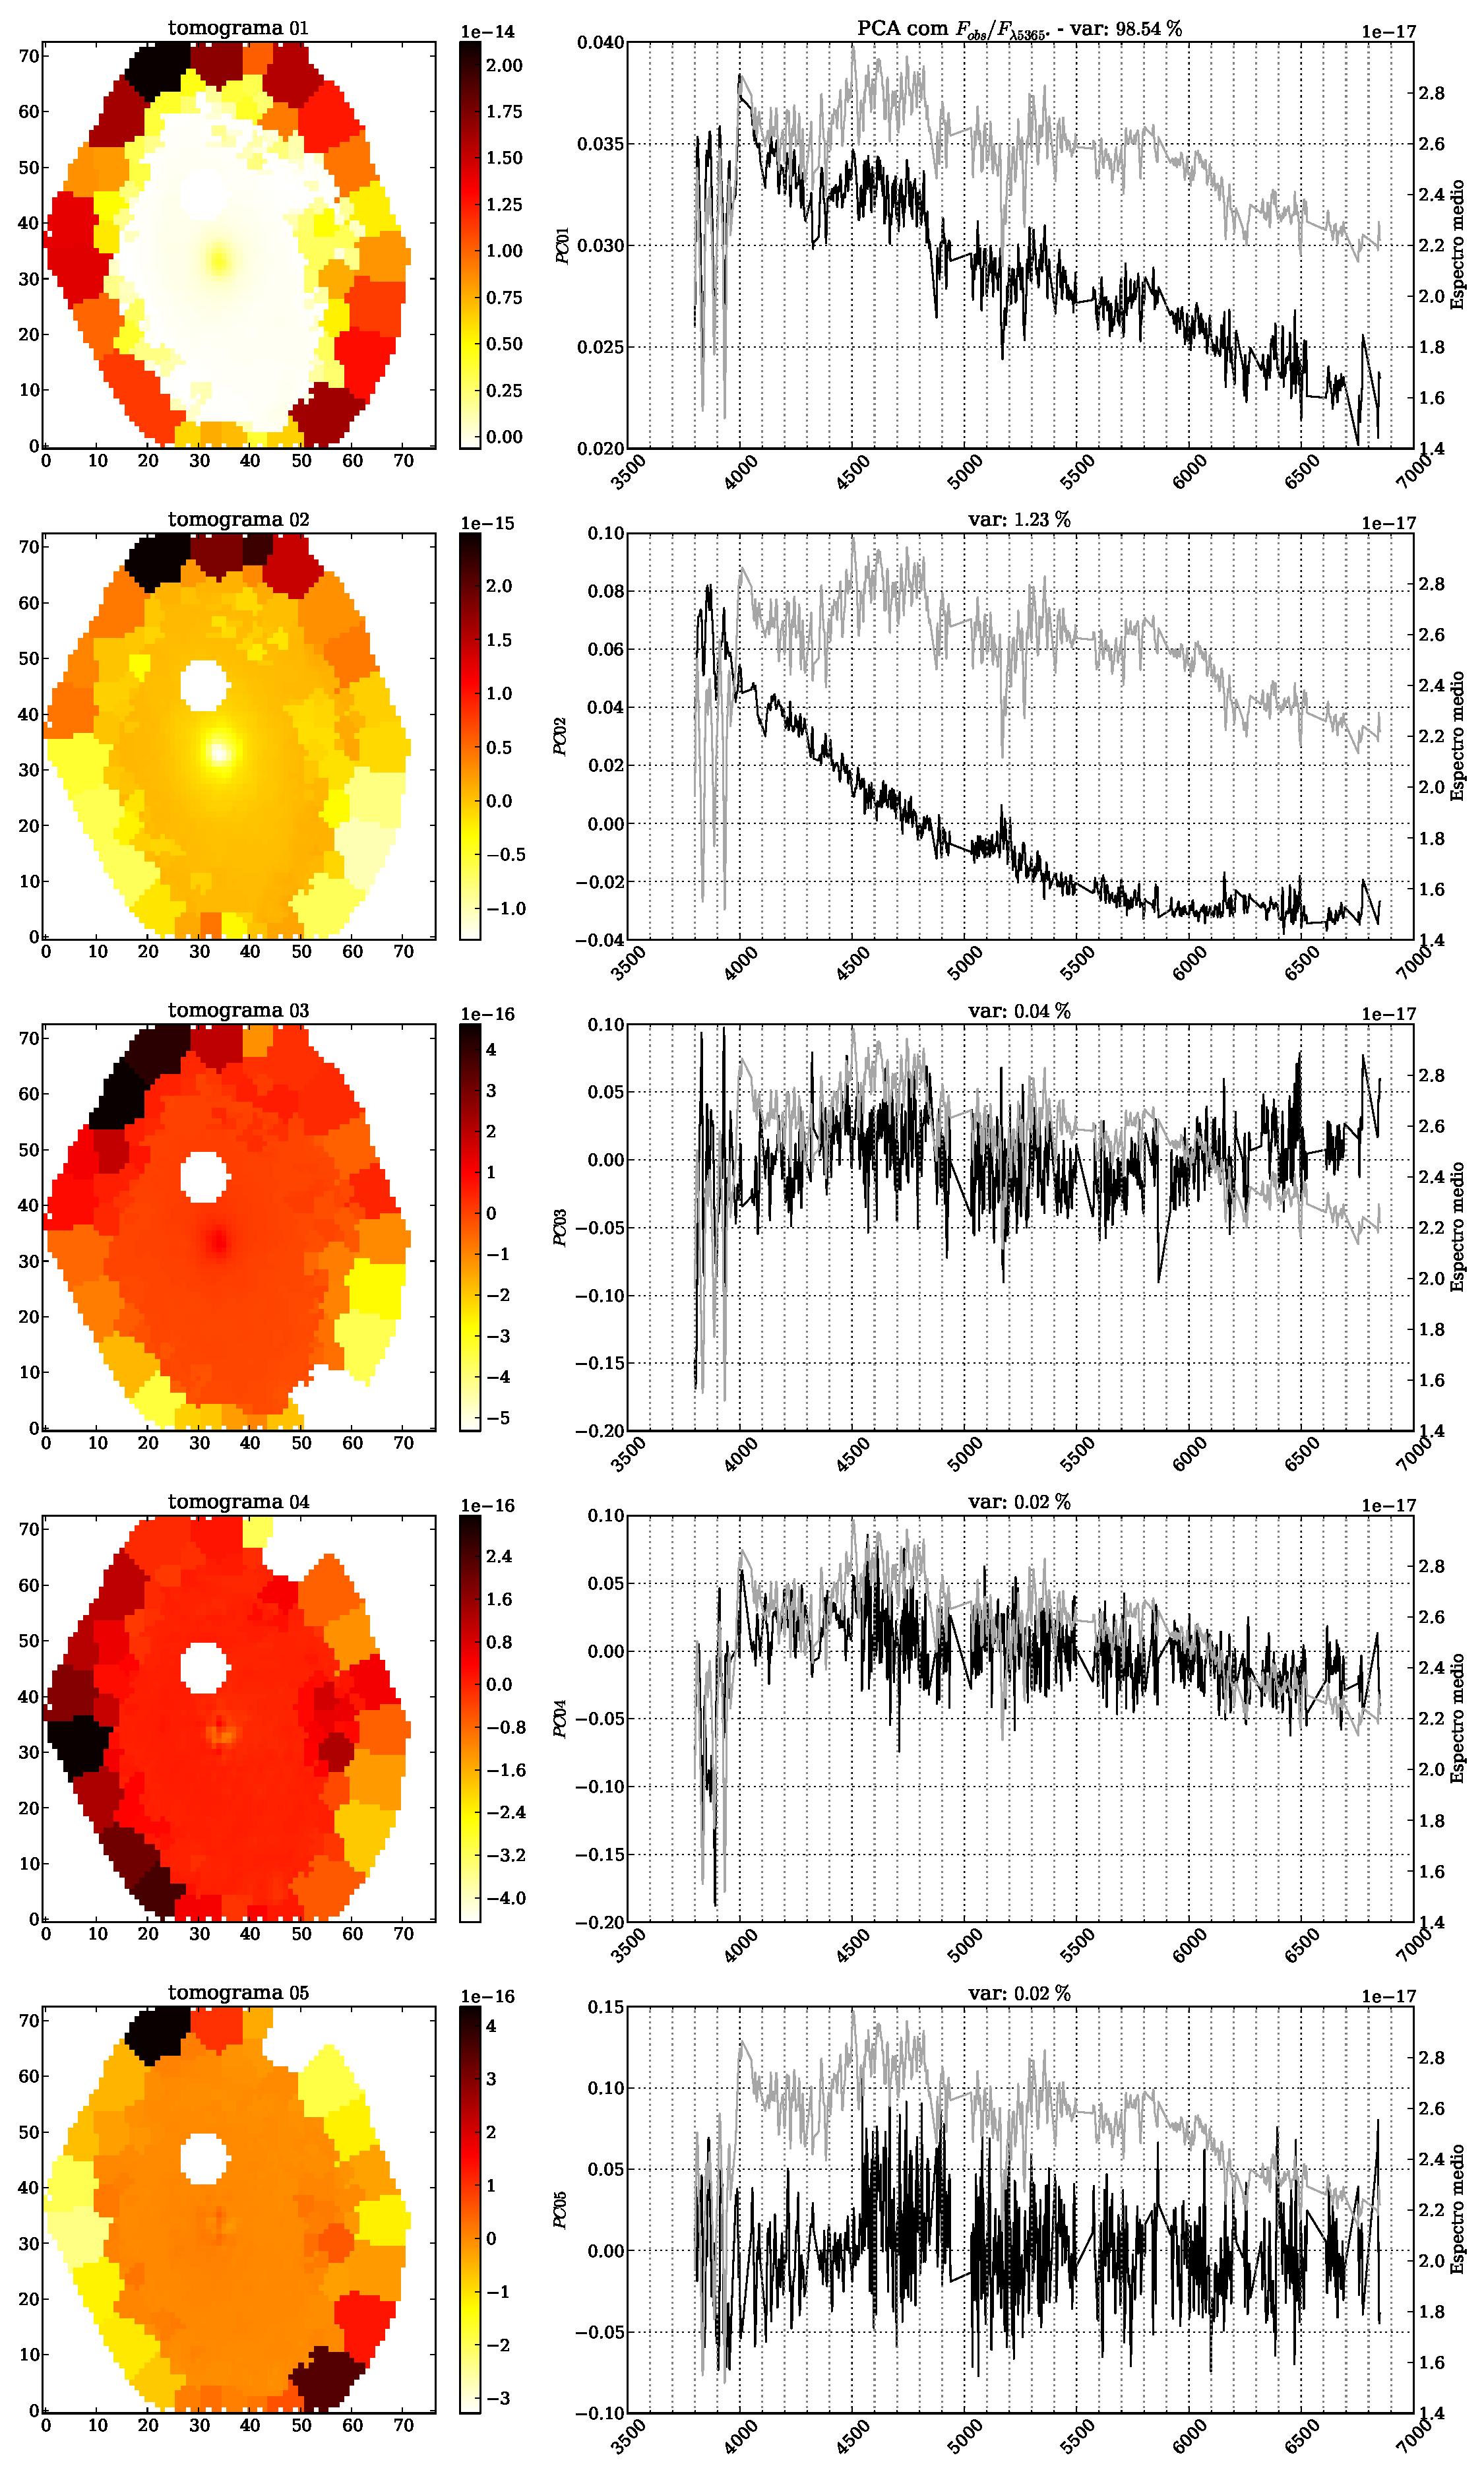
\includegraphics[width=0.9\textwidth]{figuras/K0277-tomo-obs.pdf}
    \caption[Tomogramas de 1 a 5 da gal\'axia NGC 2916 - $F_{obs}$.]
    {Cinco primeiras PCs (e seus respectivos tomogramas) resultantes da Tomografia PCA aplicado aos espectros sem
    normalização da galáxia NGC 2916.}
    \label{fig:cap4:K277tomofobs}
\end{figure}
\begin{figure}
    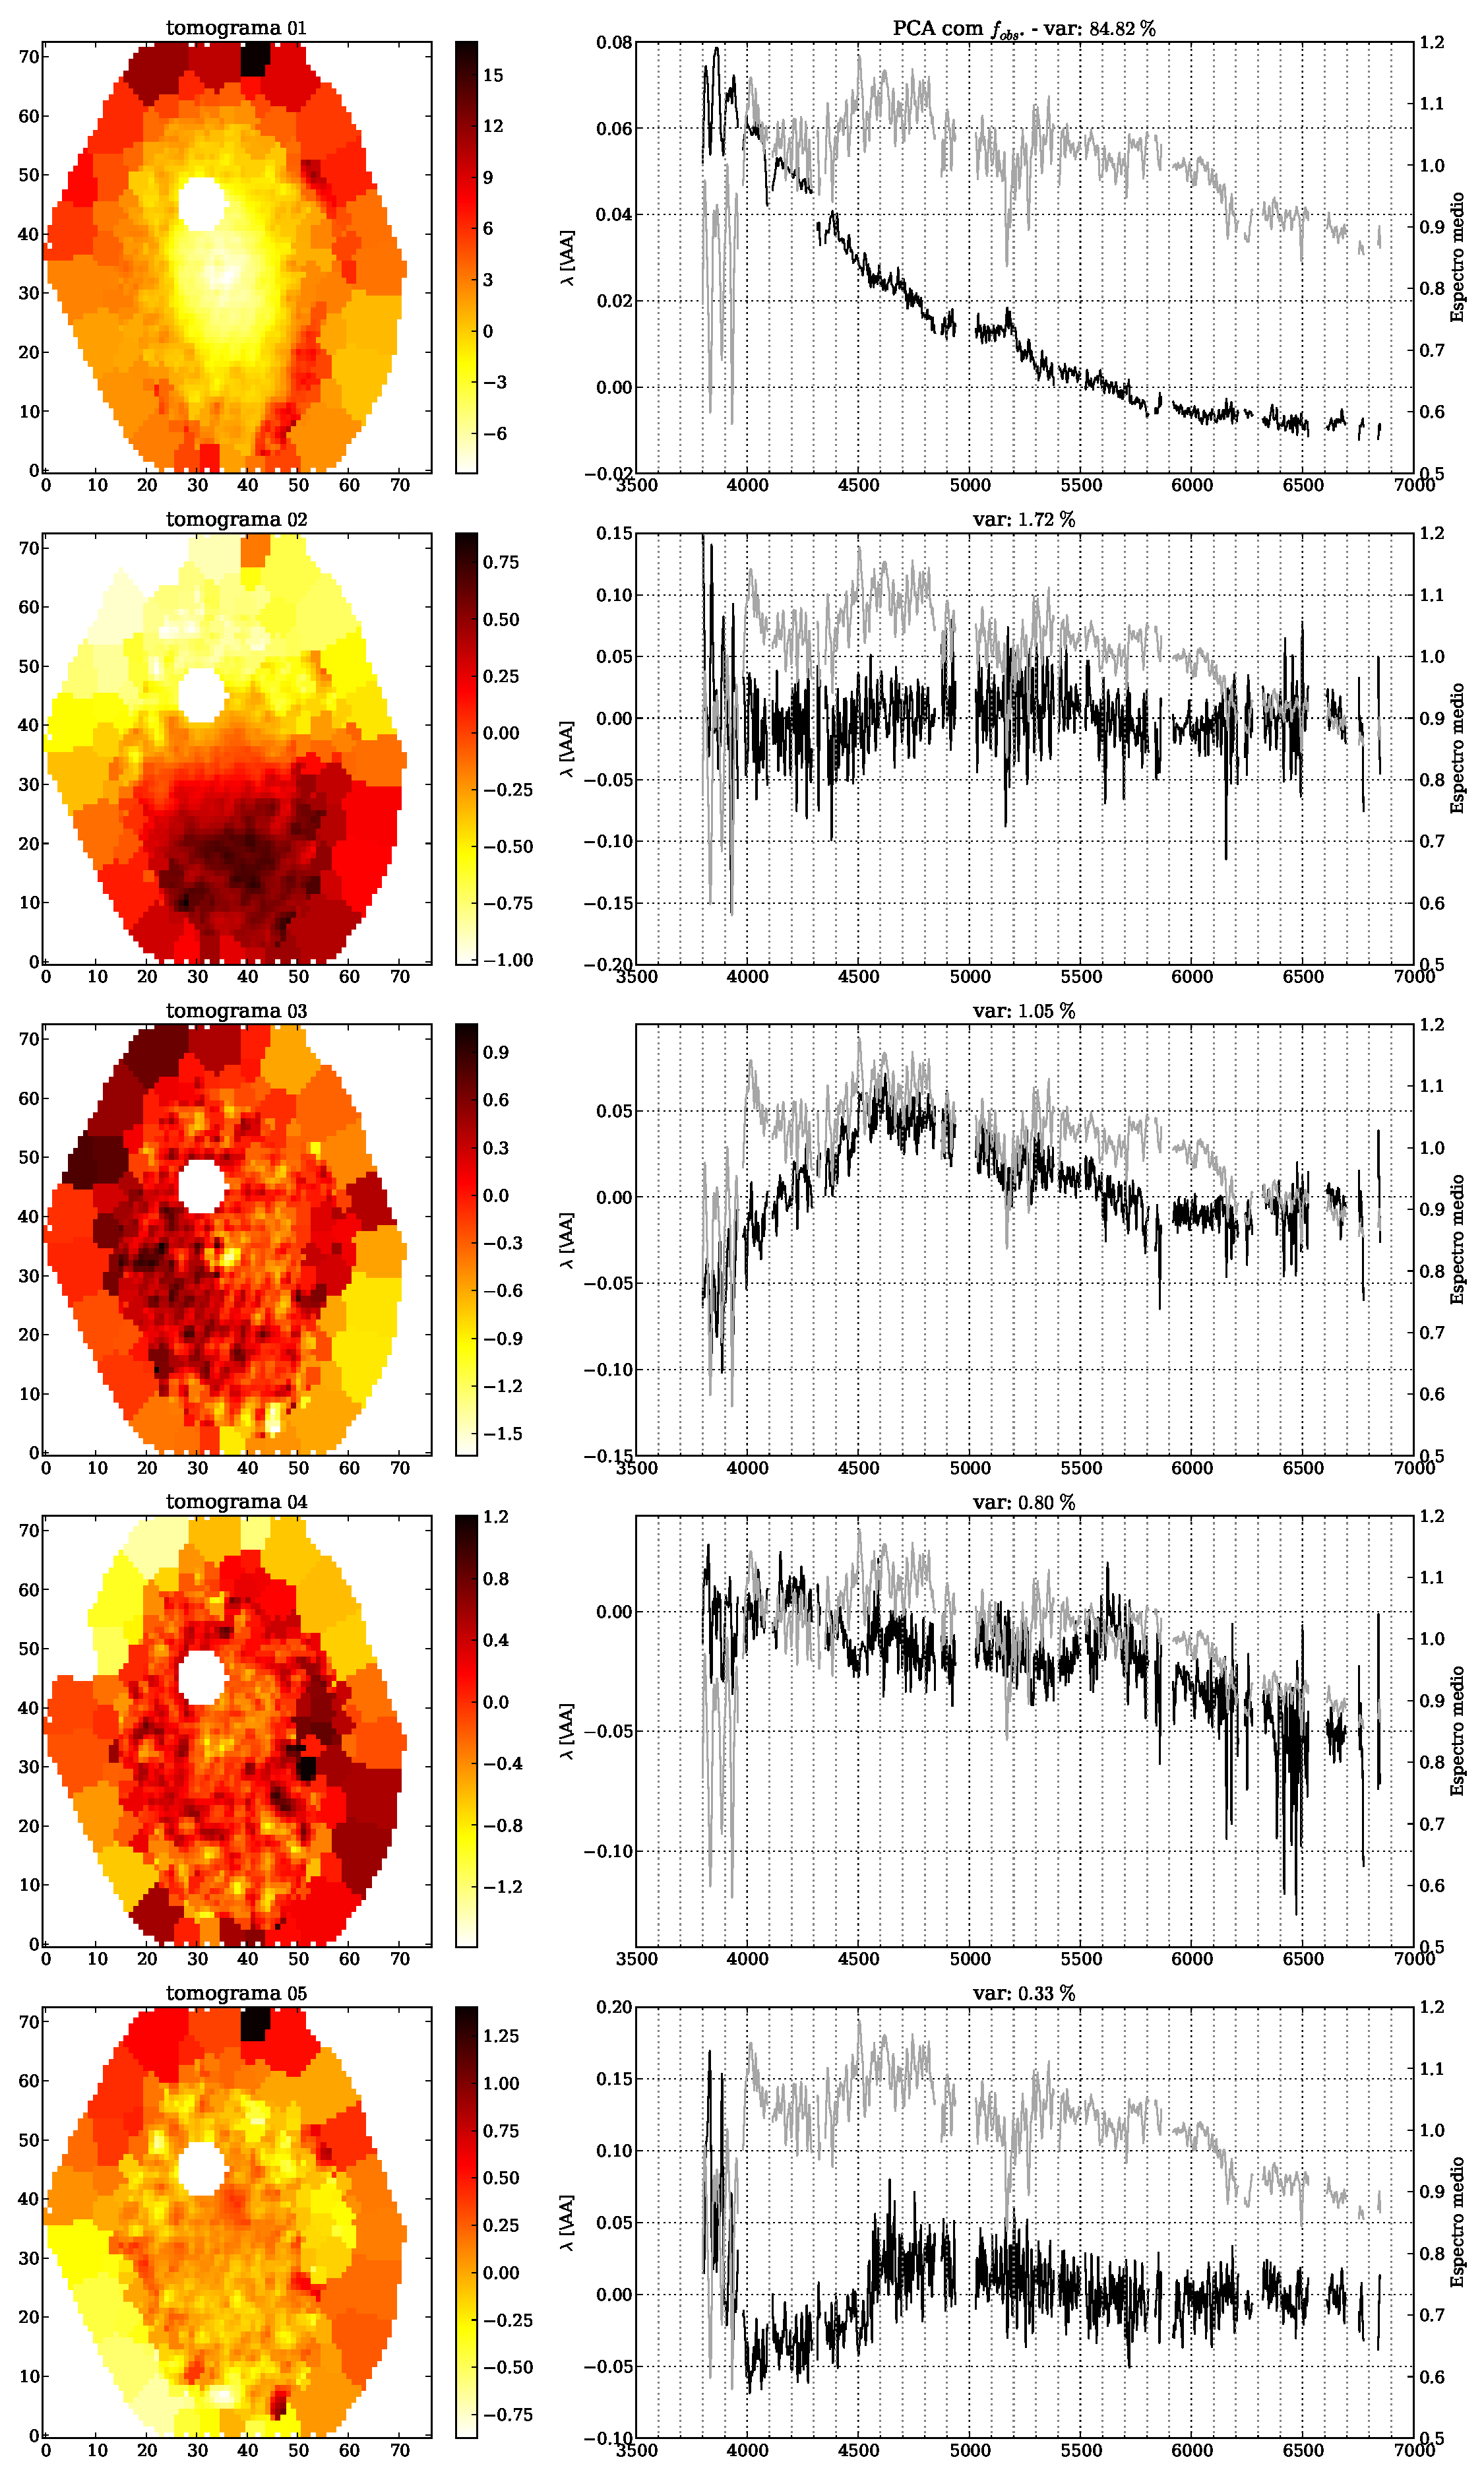
\includegraphics[width=0.9\textwidth]{figuras/K0277-tomo-obs-norm.pdf}
    \caption[Tomogramas de 1 a 5 da gal\'axia NGC 2916 - $F_{obs} / F_{\lambda 5365}$.]
    {Cinco primeiras PCs (e seus respectivos tomogramas) resultantes da Tomografia PCA aplicado aos espectros com
    normalização da galáxia NGC 2916.}
    \label{fig:cap4:K277tomofobsnorm}
\end{figure}

\begin{figure}
    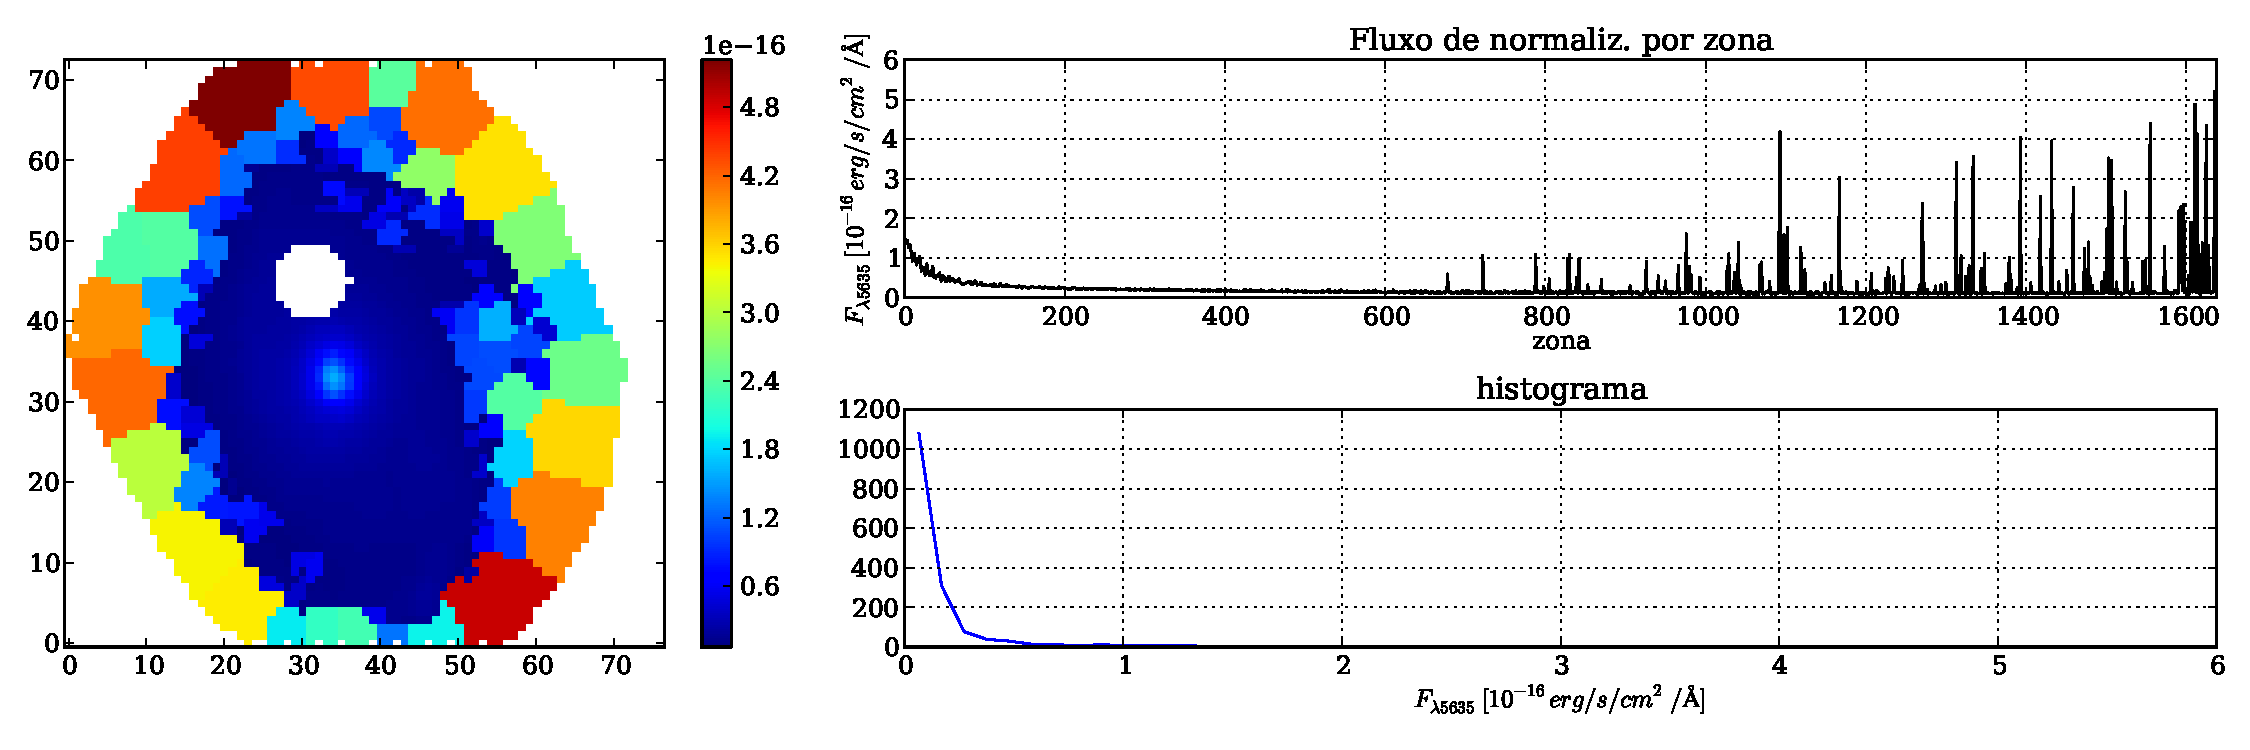
\includegraphics[width=1.\textwidth]{figuras/K0277-fobs_norm.pdf}
    \caption[Fluxos de normalização para cada zona da galáxia K0277.]
    {A imagem à esquerda e a superior direita, mostram o fluxo usado para a normalização de cada espectro em
    cada pixel (à esquerda) ou zona (superior direita). Na imagem inferior direita temos um histograma para valores do
    fluxo de normalização.}
    \label{fig:cap4:K277fobsnorm}
\end{figure}

\section{Fluxos observados e sintéticos}
\label{sec:cap4:OBSxSYN}

Com o resultado da síntese de populações estelares já organizado para as galáxias do CALIFA, realizamos o PCA no cubo de
espectros observados e no de espectros sintéticos. A grande diferença é que nos espectros sintéticos estão contidas
apenas as informações sobre populações estelares\footnote{Suavização, correções por poeira e cinemática também são
feitas nos espectros no processo de síntese. Mais detalhes em \citet{CidFernandes2005}}. Como os espectros sintéticos
não possuem as assinaturas dos equipamentos observacionais, dos processos para subtração do céu, ruídos e afins, quando
analisadas pela técnica de PCA vemos que as informações se condensam em menos PCs. Comparando os dois {\em scree tests}
na Figura \ref{fig:cap4:K0277scree} vemos que para o caso com os espectros sintéticos a curva converge mais rápido ao
zero de variância, mostrando que temos as informações mais compactadas nas primeiras PCs quando comparadas ao caso com
os espectros observados. Observando o caso sem normalização, plotado no gráfico com linha pontilhada, vemos que o efeito
causado pelo fator de escala (PC1) diminui a ``importância'' (i.e., variância) das demais PCs. As cinco primeiras PCs e
seus tomogramas provenientes do cubo com os fluxos sintéticos normalizados da galáxia NGC 2916 aparecem na Figura
\ref{fig:cap4:K277tomofsynnorm}.

\begin{figure}
    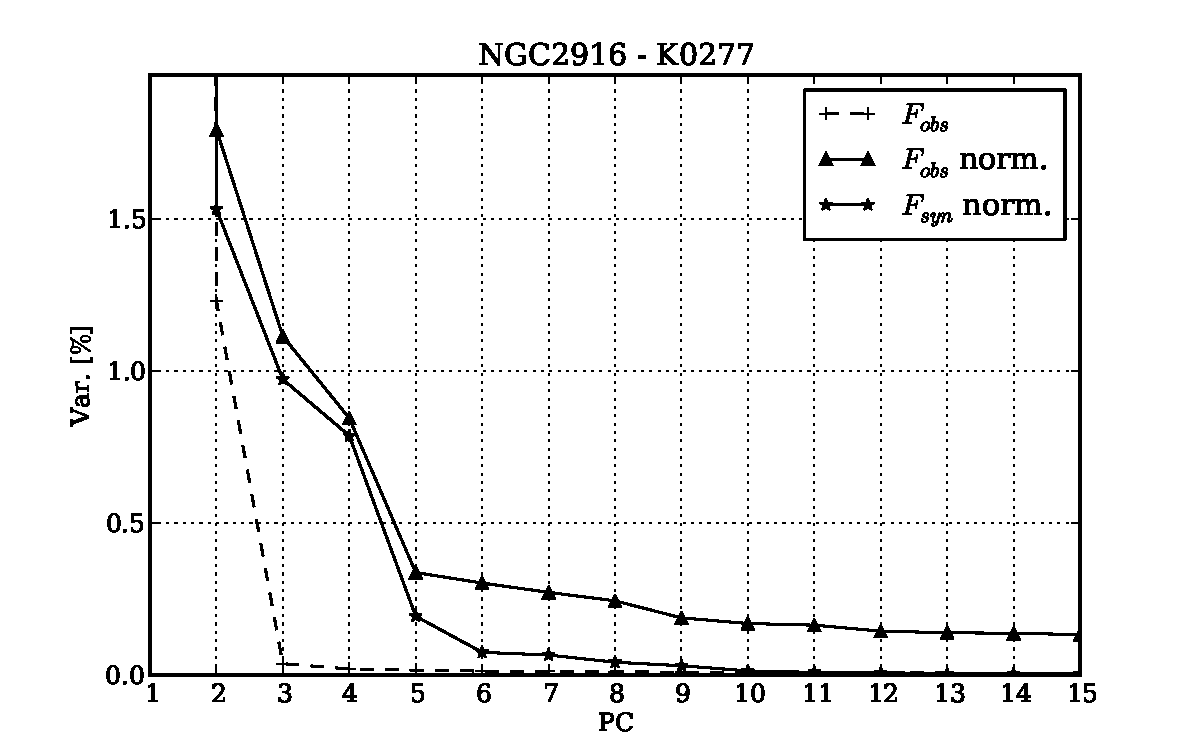
\includegraphics[width=1.\textwidth]{figuras/K0277-screetest.pdf}
    \caption[Scree test comparativo entre 3 PCAs.]
    {Scree test para 3 análises PCA da galáxia NGC 2916 (CALIFA 277). Com marcações de triângulos vemos as PCs
    resultantes do PCA com os espectros observados normalizados. As variâncias das PCs marcadas com estrela representam
    o PCA com os espectros sintéticos normalizados. Para comparação plotamos as PCs do caso sem normalização usando
    linha pontilhada.}
    \label{fig:cap4:K0277scree}
\end{figure}

Comparando os dois vemos que os resultados para os espectros sintéticos parecem ser mais ``limpos'', pois não existem
ruídos. E são! Como são espectros gerados a partir de uma base teórica para diferentes idades e metalicidades de
populações estelares, também não possuem nenhuma assinatura instrumental. Por esse fato acabamos descobrindo uma
assinatura presente em quase todas as componentes geradas pelo PCA usando os dados observados. Como comentamos no
Capítulo \ref{sec:CALePyC:Apresent} utilizamos o cubo de dados COMBO, gerado a partir da união do V500 com o V1200. Como
os espectros V1200 possuem espectros com maior resolução do que os do V500 (V1200 - FWHM $\sim 2.3$ \AA; V500 - FWHM
$\sim 6$ \AA), o processo de criação do COMBO deixa vestígios. Para essa galáxia, a junção entre os dois cubos (V500 e
V1200) para a formação do COMBO acontece exatamente nesse intervalo de comprimento de onda ($\sim 4550$ \AA). A PC5 da
Figura \ref{fig:cap4:K277tomofobsnorm} mostra um degrau grande entre $4500$ e $4600$ \AA o qual parece mostrar essa
diferença de comportamento entre as duas versões originais antes da formação do COMBO. Nessa componente fica mais
evidente, mas traçando uma linha imaginária verticamente por esse comprimento de onda fica mais fácil de perceber uma
diferença de comportamento nos dados. Já nas componentes sintéticas\footnote{Componentes geradas pelo PCA nos cubos de
espectros sintéticos.} não se vê essa mudança de comportamento no autoespectro.

A cinemática também adiciona uma variância descartável aos dados. Usando novamente a ideia da galáxia hipotética com
apenas uma população estelar, imagine agora que elas estão distribuídas uniformemente, mas estão em rotação com a
galáxia. Como anteriormente, o espectro de todos os píxels será igual, mas agora terá deslocamentos em $\lambda$. Esses
efeitos cinemáticos não estão nos trazendo informação alguma para o estudo das populações estelares. Causam um grande
disperdício de variâncias, sempre aparecendo nas primeiras PCs. Uma manipulação através do vetor de população\footnote{O
vetor de população diz o quanto de cada tipo de estrela entra na receita para construir o espectro sintético.} criado
pela síntese, juntamente com os espectros da base, pode nos ajudar a criar os espectros sintéticos sem nenhuma correção
por cinemática e poeira de maneira que se execute o PCA sem o disperdício de variância dessas componentes cinemáticas.
Também é importante lembrar que existem métodos mais eficazes e direcionados para a determinação de tais propriedades
cinemáticas. Nas galáxias presentes no CALIFA não poderia ser diferente, portanto os espectros aparecem com linhas
deslocadas para o azul ({\em blue-shifted}) ou para o vermelho ({\em red-shifted}) dependendo da velocidade de rotação
projetada. A disperção de velocidades em cada ponto da galáxia também pode causar alargamento ou estreitamento das
linhas.

\begin{figure}
    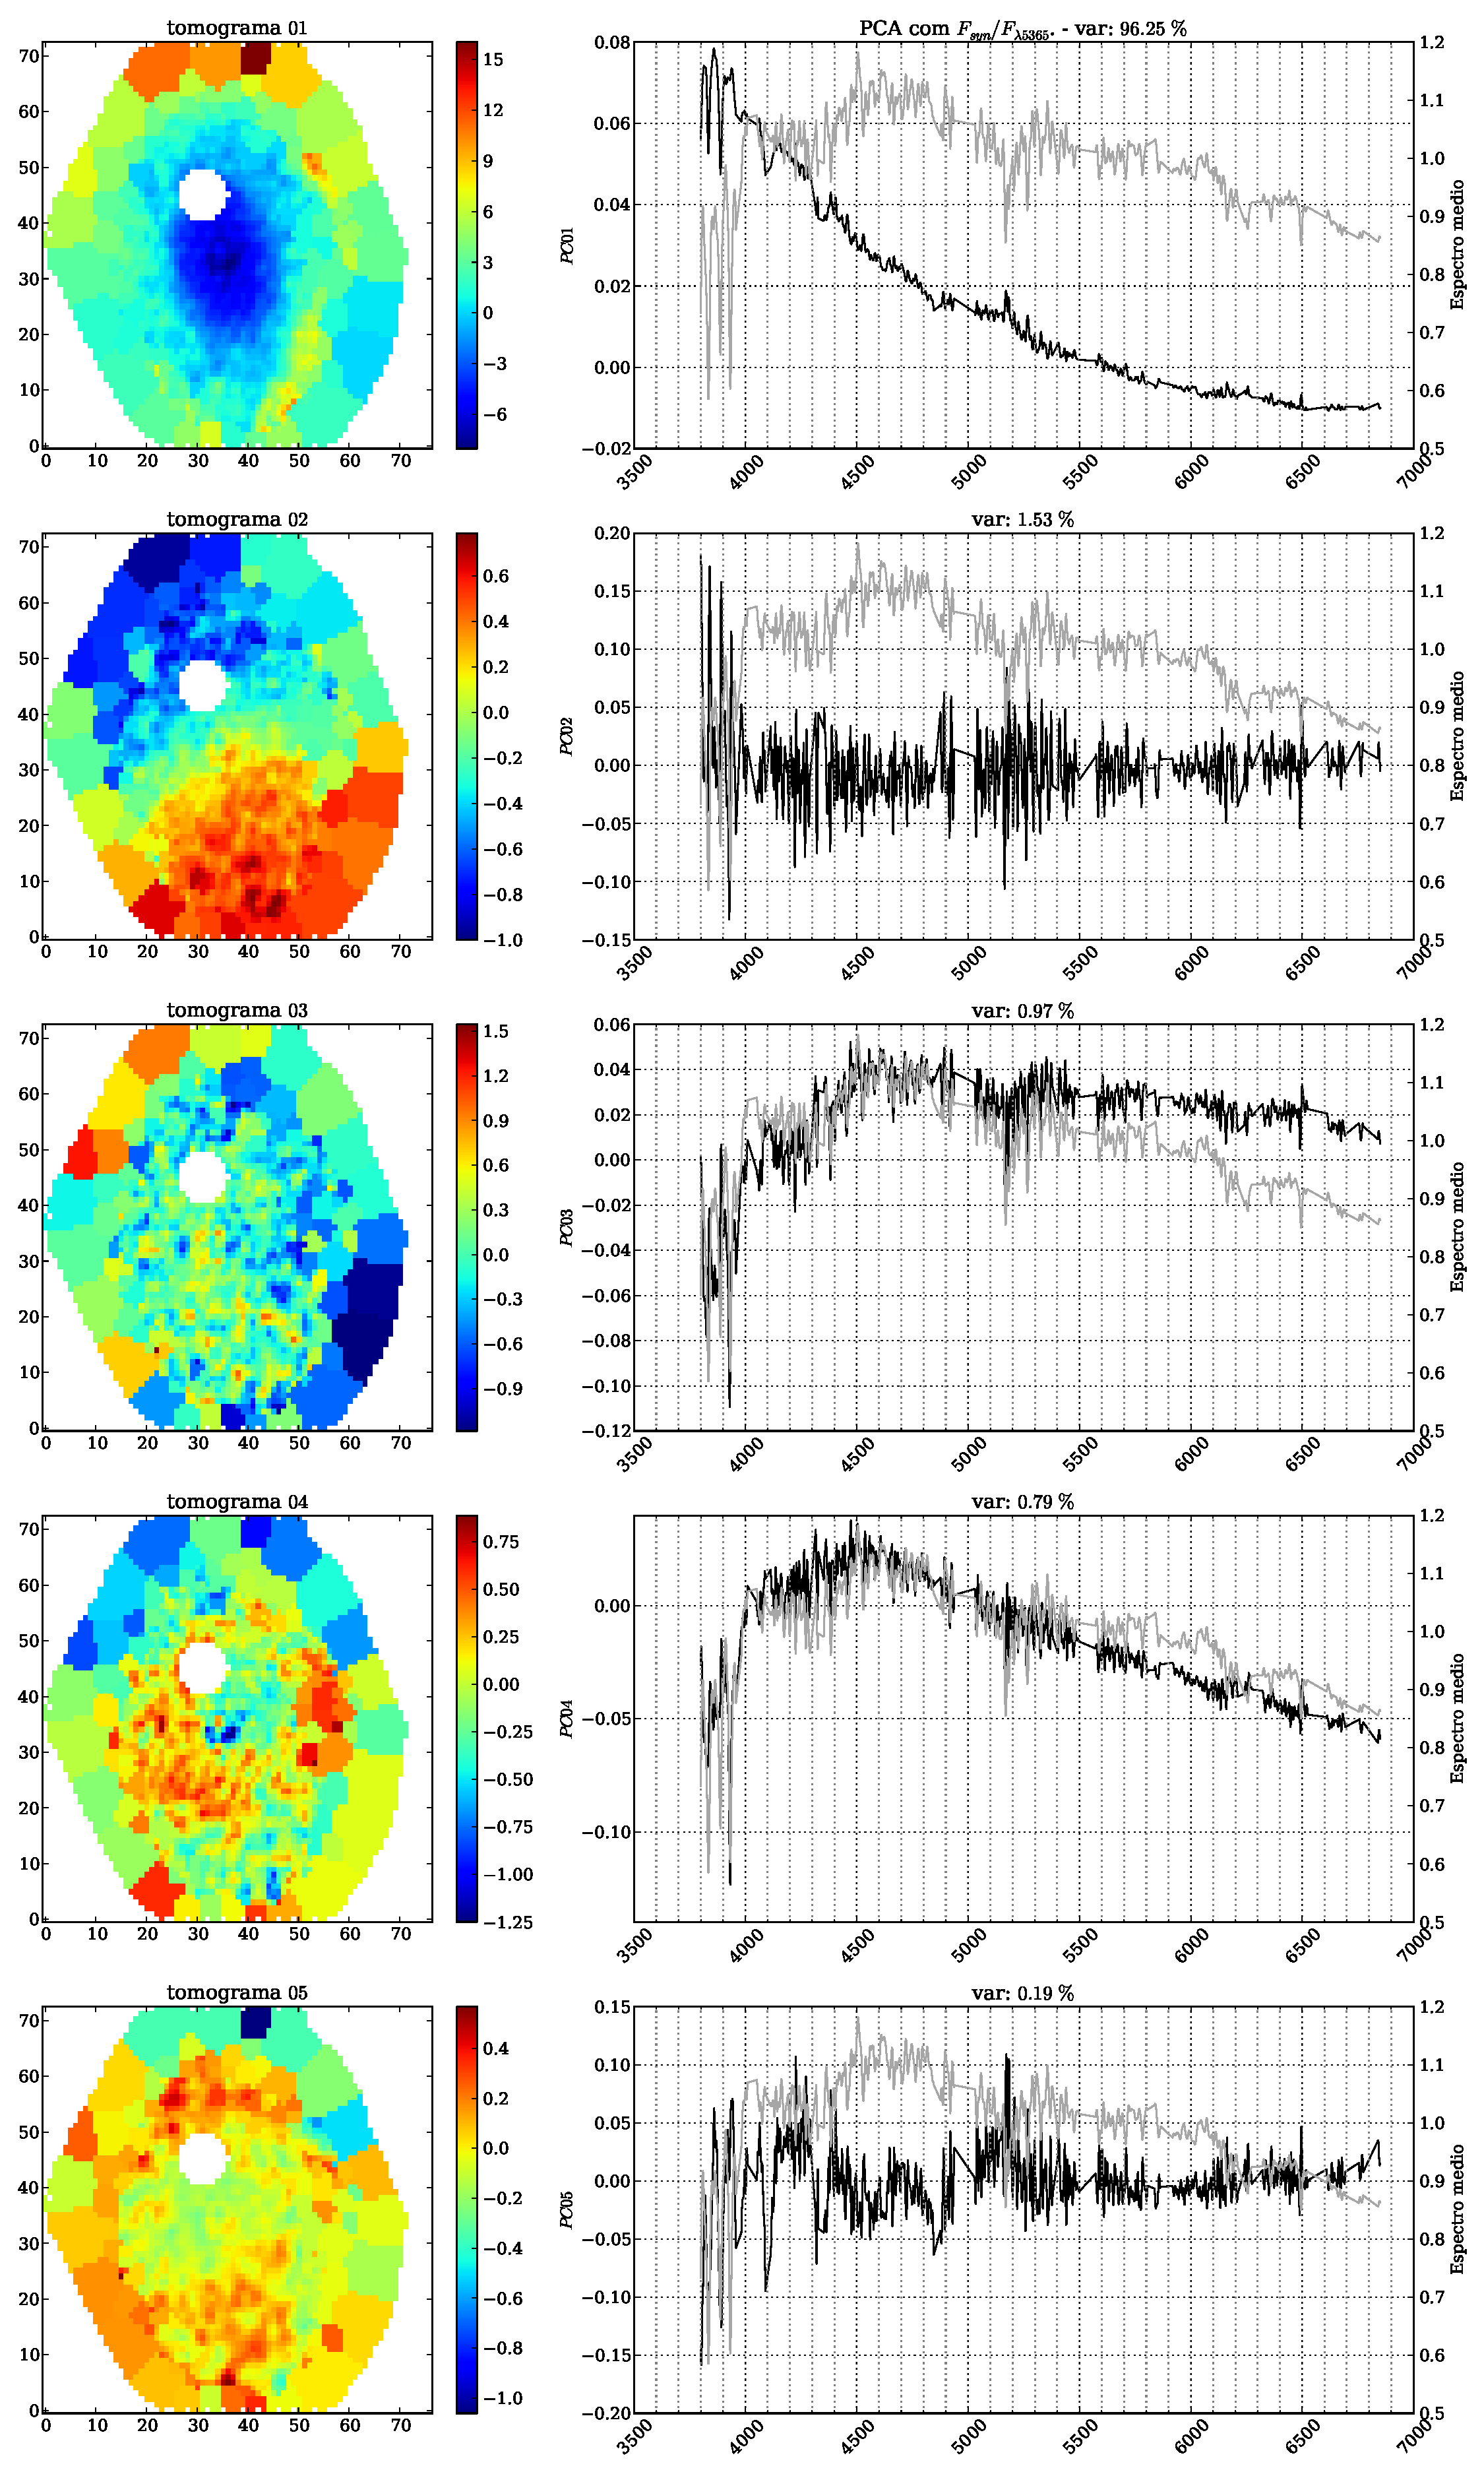
\includegraphics[width=0.9\textwidth]{figuras/K0277-tomo-syn-norm.pdf}
    \caption[Tomogramas de 1 a 5 da gal\'axia NGC 2916 - $F_{syn} / F_{\lambda 5365}$ .]
    {Cinco primeiras PCs (e seus respectivos tomogramas) resultantes da Tomografia PCA aplicado aos espectros
    sintéticos normalizados da galáxia NGC 2916.}
    \label{fig:cap4:K277tomofsynnorm}
\end{figure}

\section{Comparando as PCs com o \STARLIGHT: engenharia reversa}
\label{sec:cap4:EngRev}

Descobrir o sentido físico de cada PC não é uma tarefa fácil. Como comentamos anteriormente, o PCA te dá a resposta, mas
você geralmente não sabe qual a pergunta. Uma forma de buscar sentido físico nas componentes é analisar as correlações
com propriedades físicas da galáxia. Com o resultado da síntese de populações estelares obtido pelo \starlight e
organizado pelo PyCASSO fica simples fazermos as correlações entre os dados na base gerada pelo PCA. Nas Figuras
\ref{fig:cap4:K0277correfobsnorm} e \ref{fig:cap4:K0277correfsynorm} vemos as correlações entre vários parâmetros
físicos e o peso de cada PC por zona (tomograma versus parâmetro físico).

A Figura \ref{fig:cap4:K0277correfobs} mostra também o efeito que a falta de normalização faz com o resultado do PCA.
Esse fator de amplitude que não é removido pela normalização se concentra principalmente na primeira PC, mas ainda
deixa vestígios se misturando com as outras PCs fazendo com que haja correlação entre as PCs e os parâmetros físicos
estudados.

\begin{figure}
    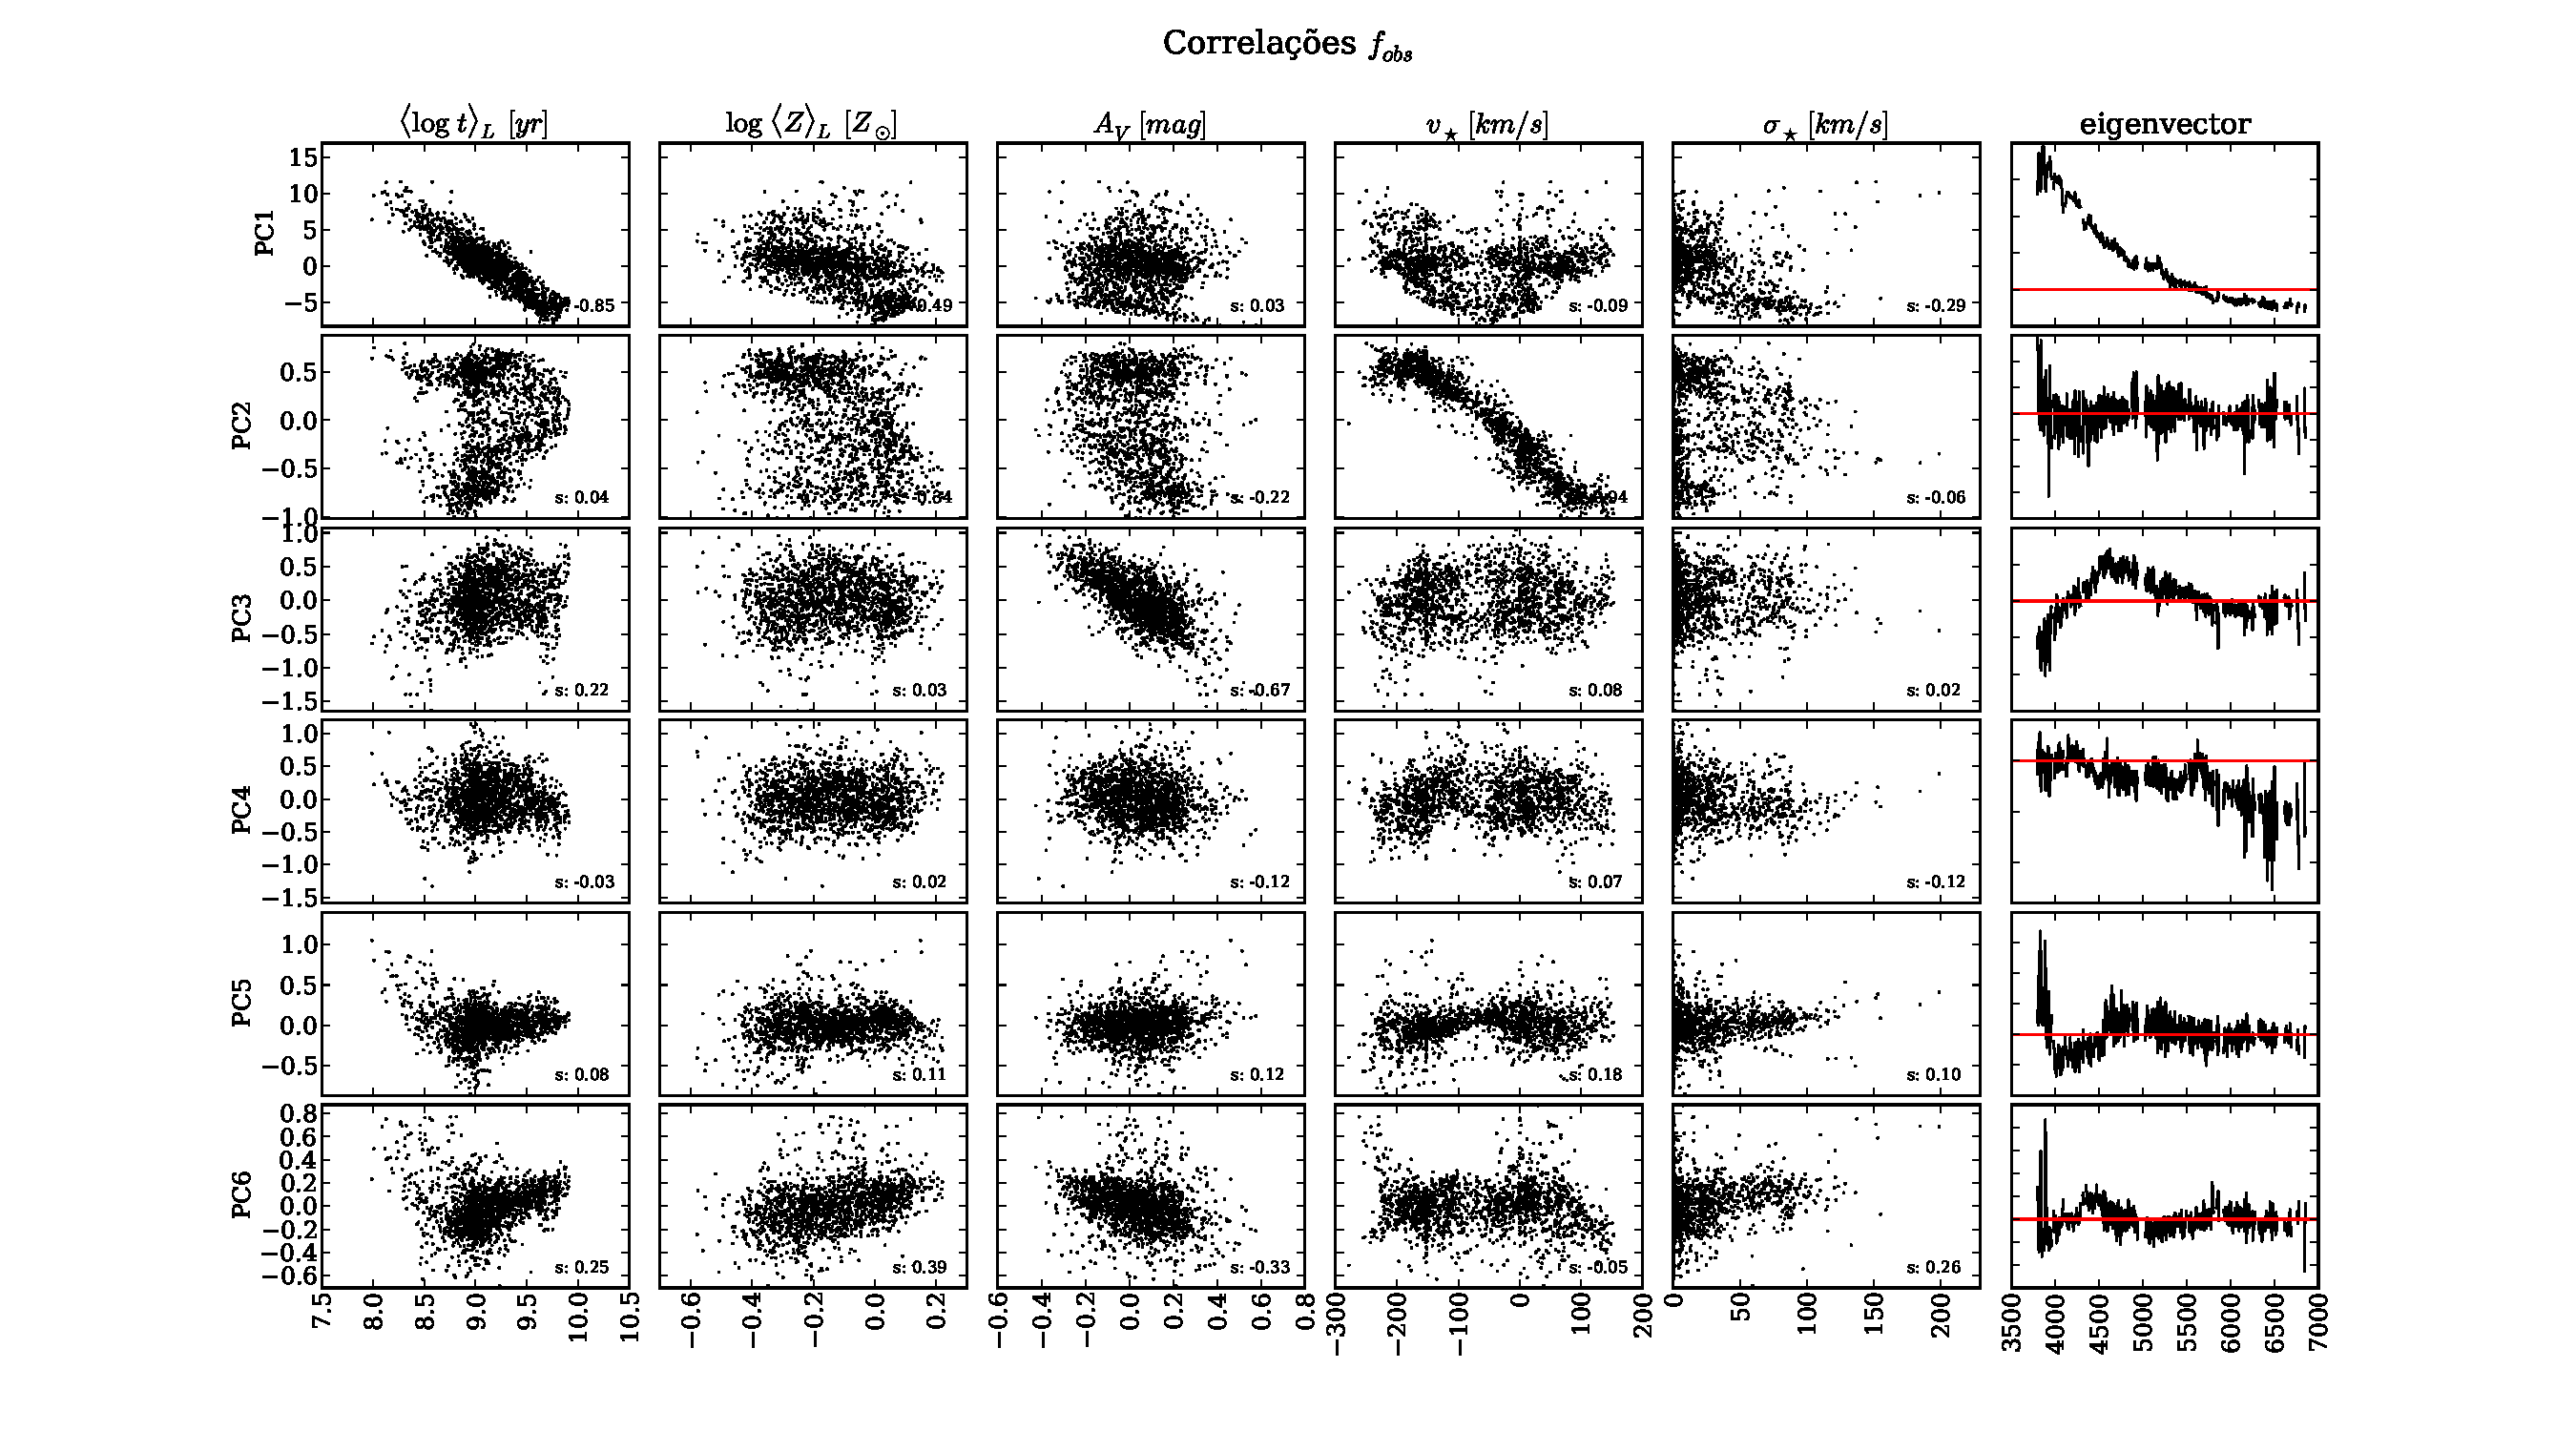
\includegraphics[width=1.4\textwidth, angle=-90]{figuras/K0277-correl-f_obs_norm-PCvsPhys.pdf}
	\caption[Correlações PCs vs. par\^ametros f\'isicos - $F_{obs}$ norm.]
    {Correlações entre os pesos por zona das seis primeiras PCs do PCA feito para o cubo com os dados observados
    normalizados e cinco parâmetros físicos.q Pela ordem de colunas da esquerda para direita temos $\log$ t, $\log$ $Z /
    Z_{\odot}$, $A_V$, $v_{\star}$, $\sigma_{\star}$. Na última coluna temos o autoespectro para ajudar na visualização.
    A linha em vermelho no gráfico do autoespectro serve para identificar o zero.}
    \label{fig:cap4:K0277correfobsnorm}
\end{figure}

\begin{figure}
    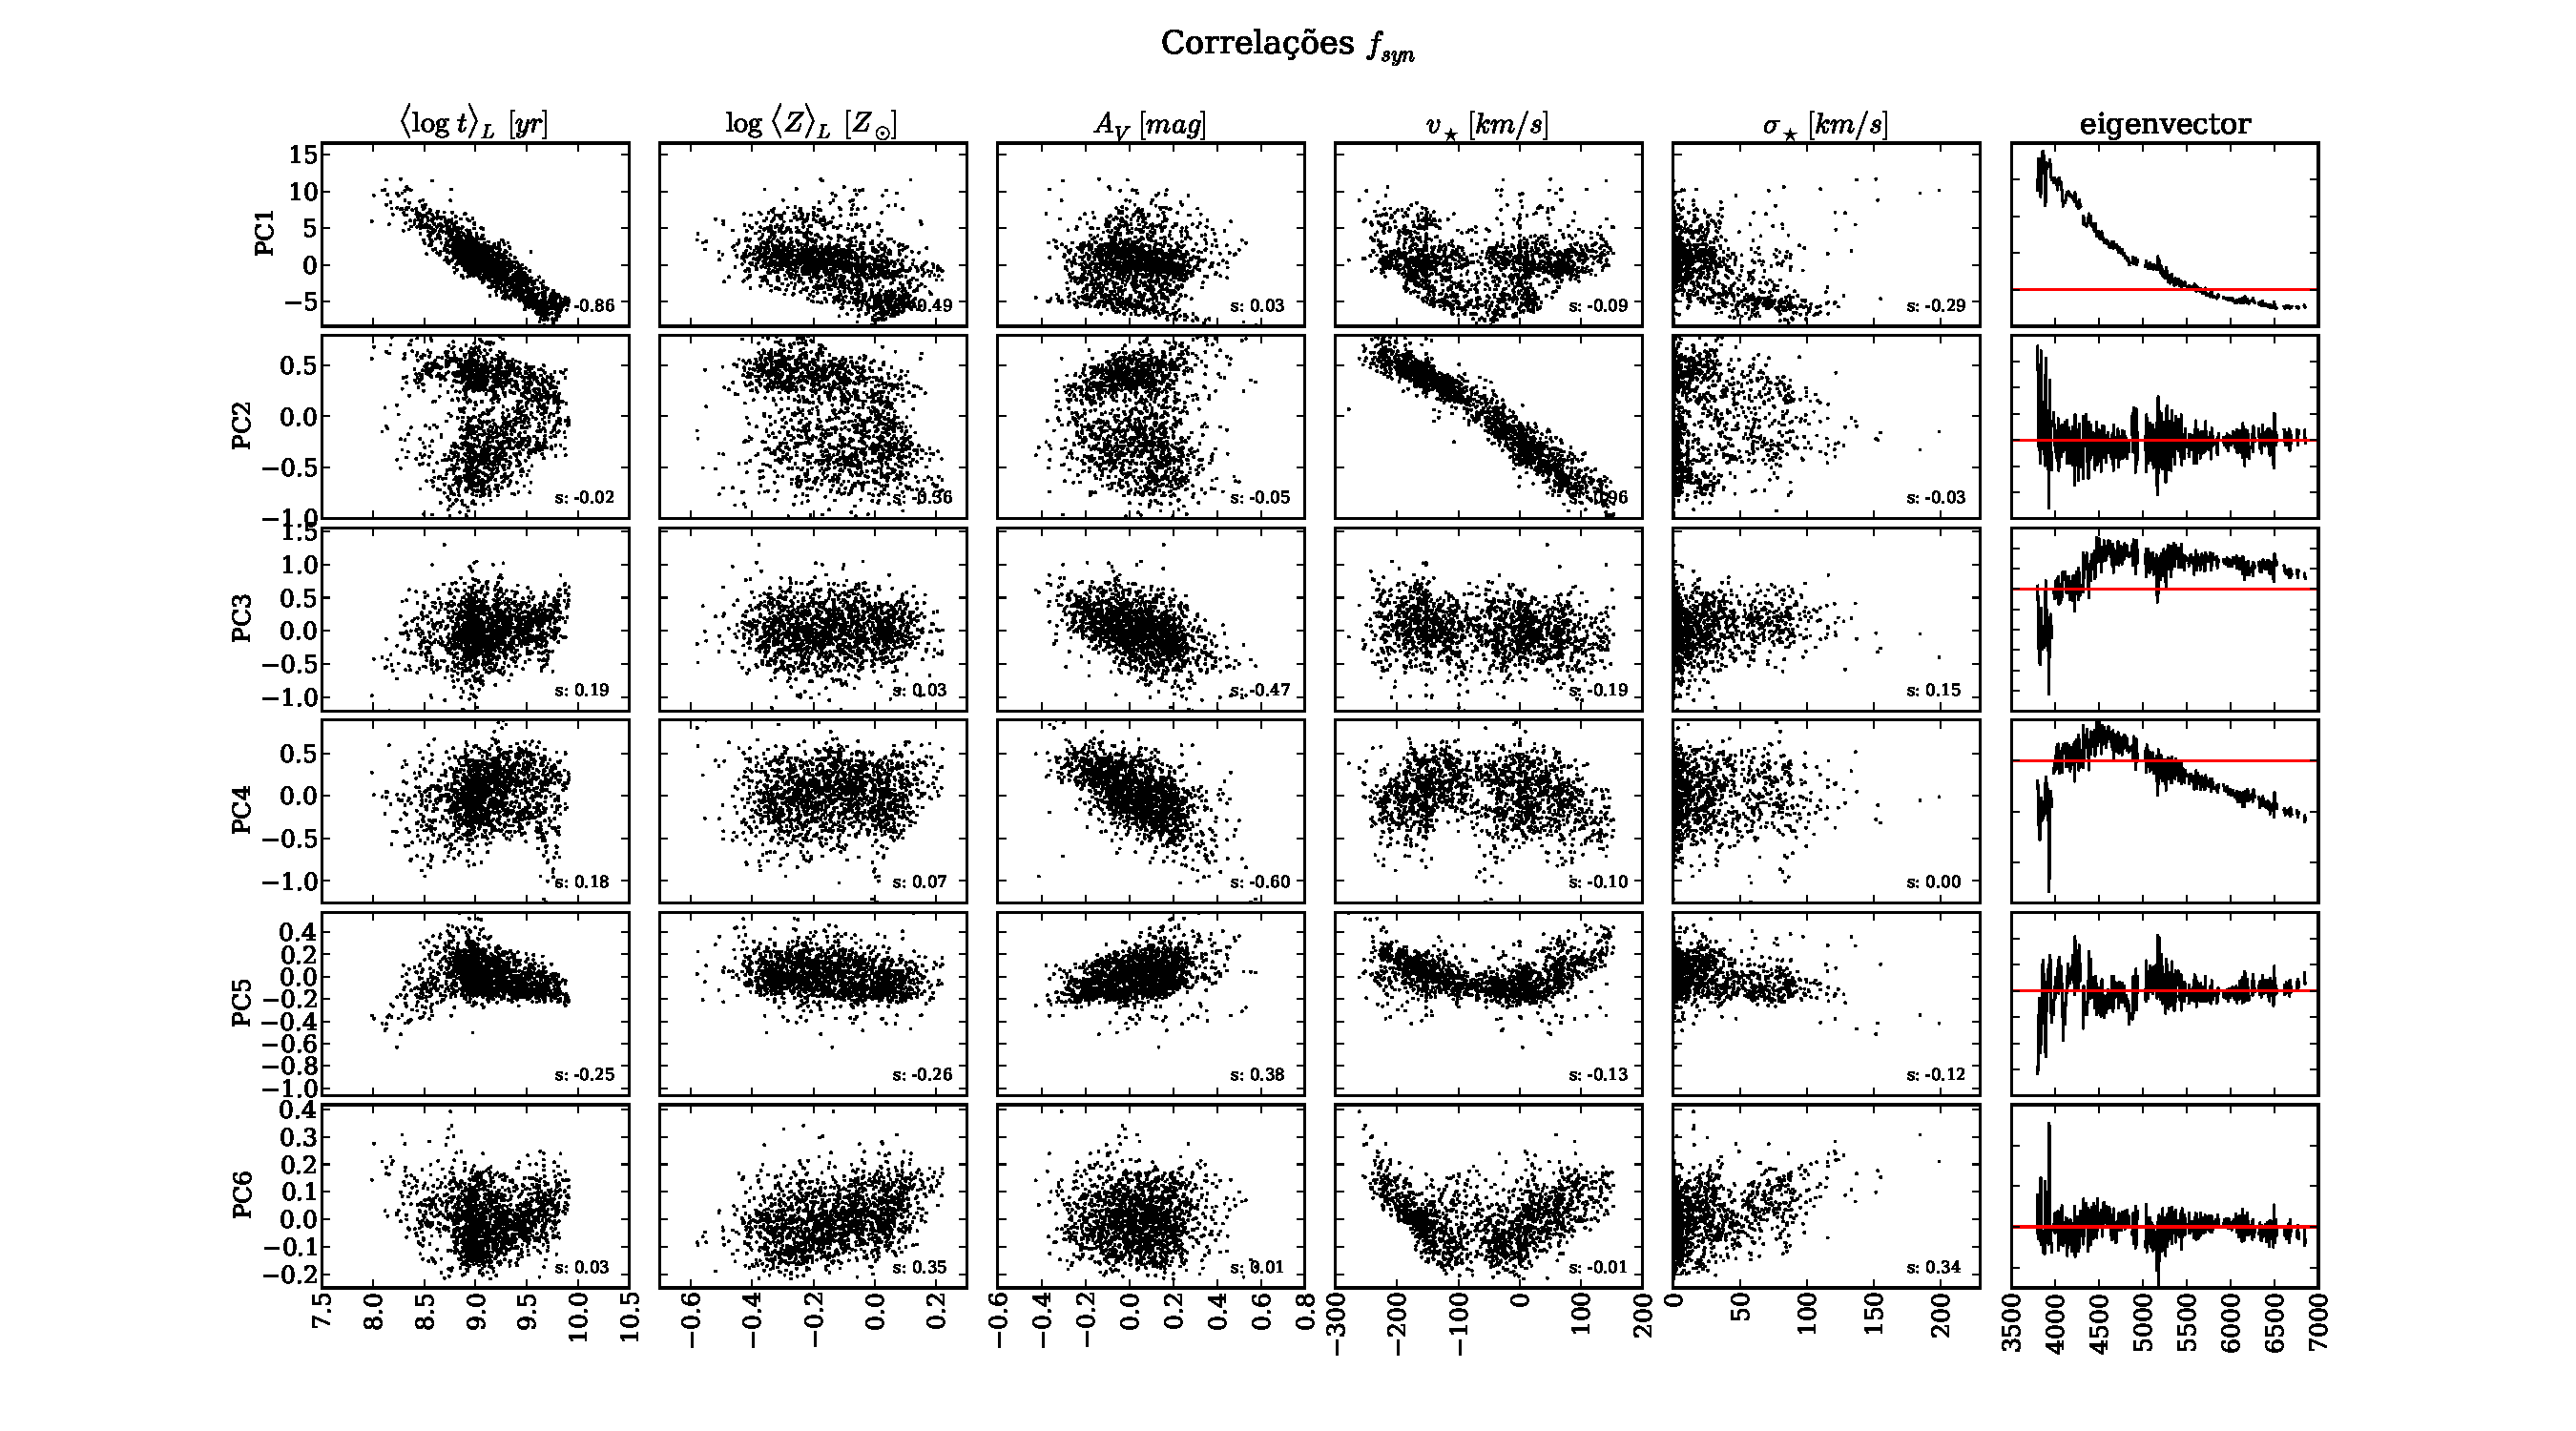
\includegraphics[width=1.4\textwidth, angle=-90]{figuras/K0277-correl-f_syn_norm-PCvsPhys.pdf}
	\caption[Correlações PCs vs. par\^ametros f\'isicos - $F_{syn}$ norm.]
    {Correlações entre os pesos por zona das seis primeiras PCs do PCA feito para o cubo com os dados sintéticos
    normalizados e cinco parâmetros físicos.q Pela ordem de colunas da esquerda para direita temos $\log$ t, $\log$ $Z /
    Z_{\odot}$, $A_V$, $v_{\star}$, $\sigma_{\star}$. Na última coluna temos o autoespectro para ajudar na visualização.
    A linha em vermelho no gráfico do autoespectro serve para identificar o zero.}
    \label{fig:cap4:K0277correfsynorm}
\end{figure}

\begin{figure}
    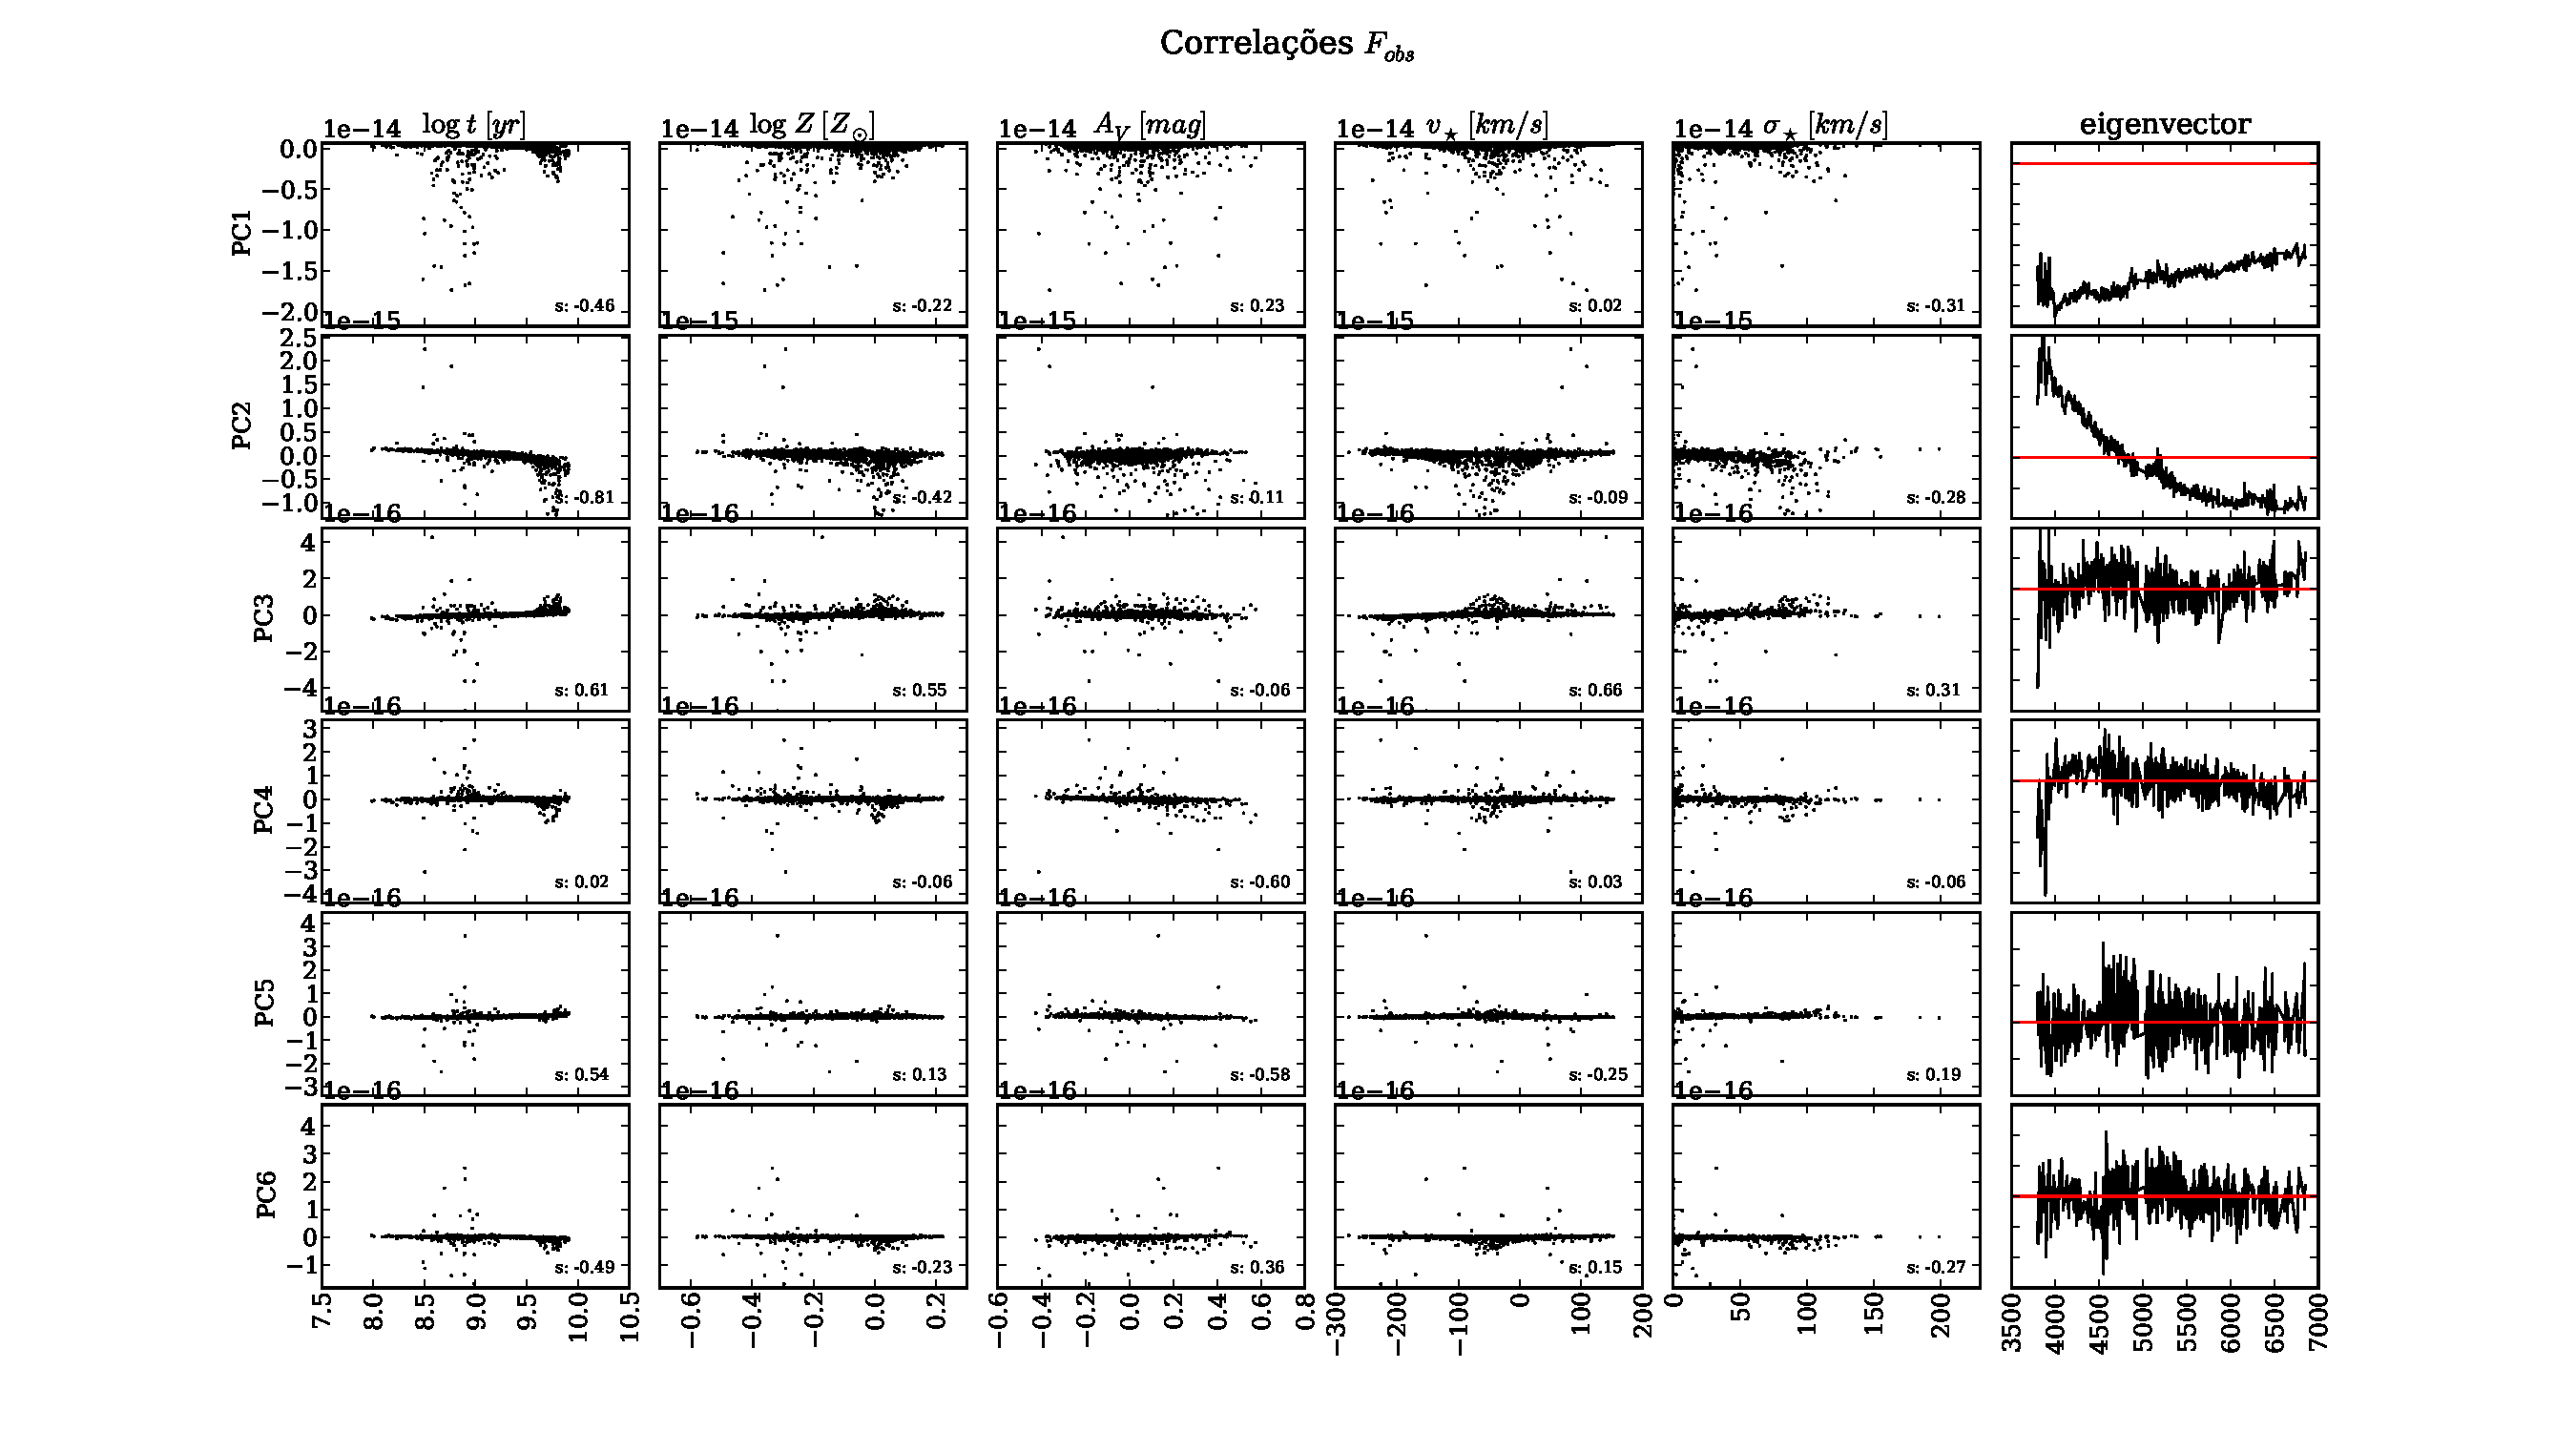
\includegraphics[width=1.4\textwidth, angle=-90]{figuras/K0277-correl-f_obs-PCvsPhys.pdf}
	\caption[Correlações PCs vs. par\^ametros f\'isicos - $F_{obs}$.]
    {Correlações entre os pesos por zona das seis primeiras PCs do PCA feito para o cubo com os dados observados e cinco
    parâmetros físicos.q Pela ordem de colunas da esquerda para direita temos $\log$ t, $\log$ $Z / Z_{\odot}$, $A_V$,
    $v_{\star}$, $\sigma_{\star}$. Na última coluna temos o autoespectro para ajudar na visualização. A linha em
    vermelho no gráfico do autoespectro serve para identificar o zero.}
    \label{fig:cap4:K0277correfobs}
\end{figure}

\ldots \dots \ldots \ldots

Caso as grandezas físicas analisadas em uma galáxia fossem não-correlacionadas seria muito mais fácil fazer uma
comparação entre PCs e grandezas físicas, mas geralmente não é o que ocorre. Para colhermos informações sobre os objetos
no céu só temos duas formas: através imagens ou de espectros. Em ambas formas, diferentes efeitos físicos causam efeitos
semelhantes nas cores (imagem) ou nos espectros. Esses efeitos fazem com que alguns dos parâmetros físicos fiquem
extremamente correlacionados.\ojo \citneed \textcolor{red}{Gostaria de adicionar aqui algumas referências como alguns
dos papers do SEAGal/Starlight que fala sobre as degenerescencias de idade e metalicidade e algumas outras grandezas
correlacionadas. Coloquei essa parte aqui pensando naquela crítica que o cara me fez lá no México sobre as grandezas em
astrofísica serem extremamente correlacionadas, mas não sei até que ponto é legal comentar sobre isso visto que
estamos analisando as coisas via correlação\ldots talvez essa discussão possa ficar mais pro Cap 6 nas conclusões.}.

\ldots \dots \ldots \ldots
                                                                                                                                                                                                                                                                               
\fixme {\bf DAQUI PRA BAIXO VAI PRO CAP 2}
Antes dos espectros chegarem ao PyCASSO, todas as informações de {\em flags}\footnote{Marcações.} em {\em bad pixels} e
linhas telúricas\footnote{Linhas de emissão ou absorção referentes à atmosfera.} são criadas em um {\em pipeline} de
pré-processamento chamado {\sc qbick}. Esse {\em pipeline} também prepara os cubos para a execução do \starlight, que
posteriormente serão organizados pelo PyCASSO, definindo as zonas de Voronoi, a reamostragem em $\lambda$ e colocando os
espectros em repouso usando o {\em redshift} calculado dentro dos $5"$ centrais da galáxia. Todas essas informações e
pré-processamentos provenientes do {\sc qbick} são herdadas pelo PyCASSO e já estão contidadas em seus cubos de
espectros.

Primeiro todos os espectros são limitados ao intervalo de $3800$ a $6850$ \AA. Após essa limitação, fazemos uma
estatística com todos os {\em bad pixels} e linhas telúricas de cada cubo e removemos qualquer um que esteja presente em
mais de $5\%$ dos espectros. Cabe aqui lembrar que todos os espectros precisam ter os mesmos pontos em comprimento de
onda pois precisamos construir a matriz de covariância. Podemos ver o efeito desses pré-processamentos nos espectros
através dos primeiro e segundo espectros na Figura \ref{fig:cap4:checkmask}.

\begin{figure}
    %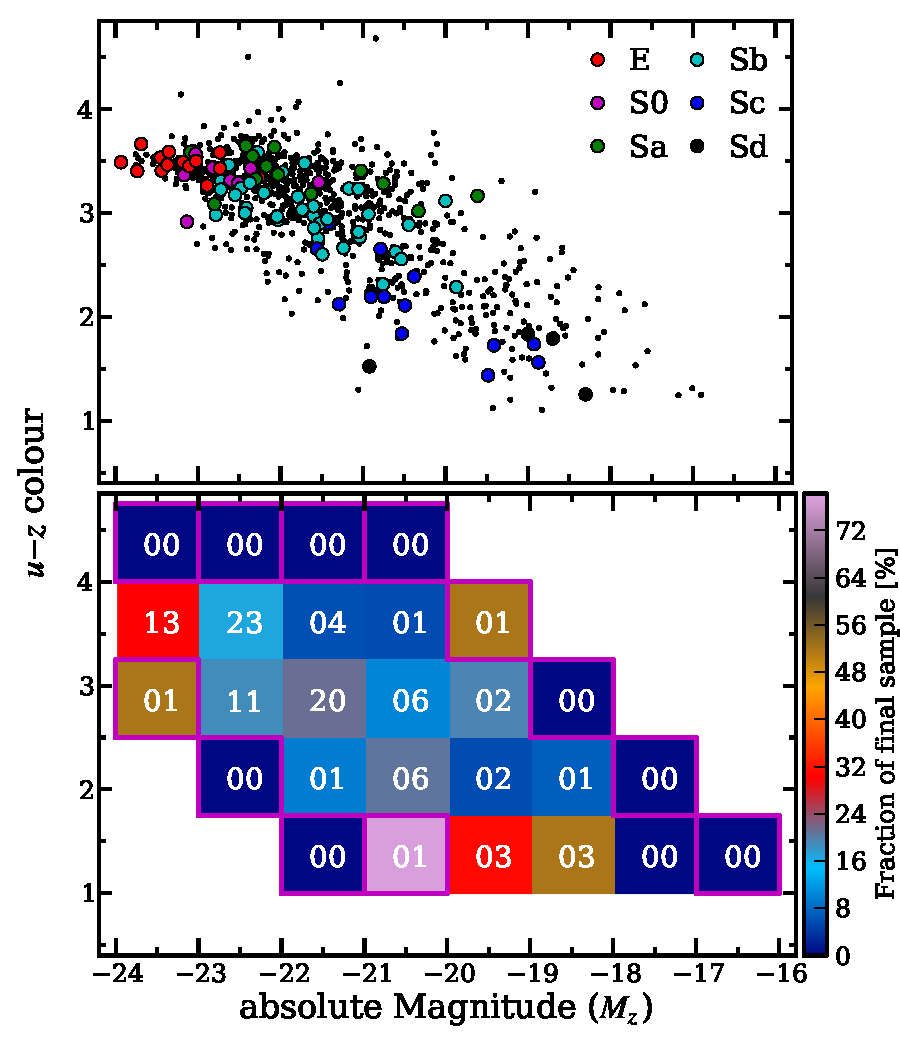
\includegraphics[height=0.5\textwidth]{figuras/figHusemann2013Fig2.pdf}
    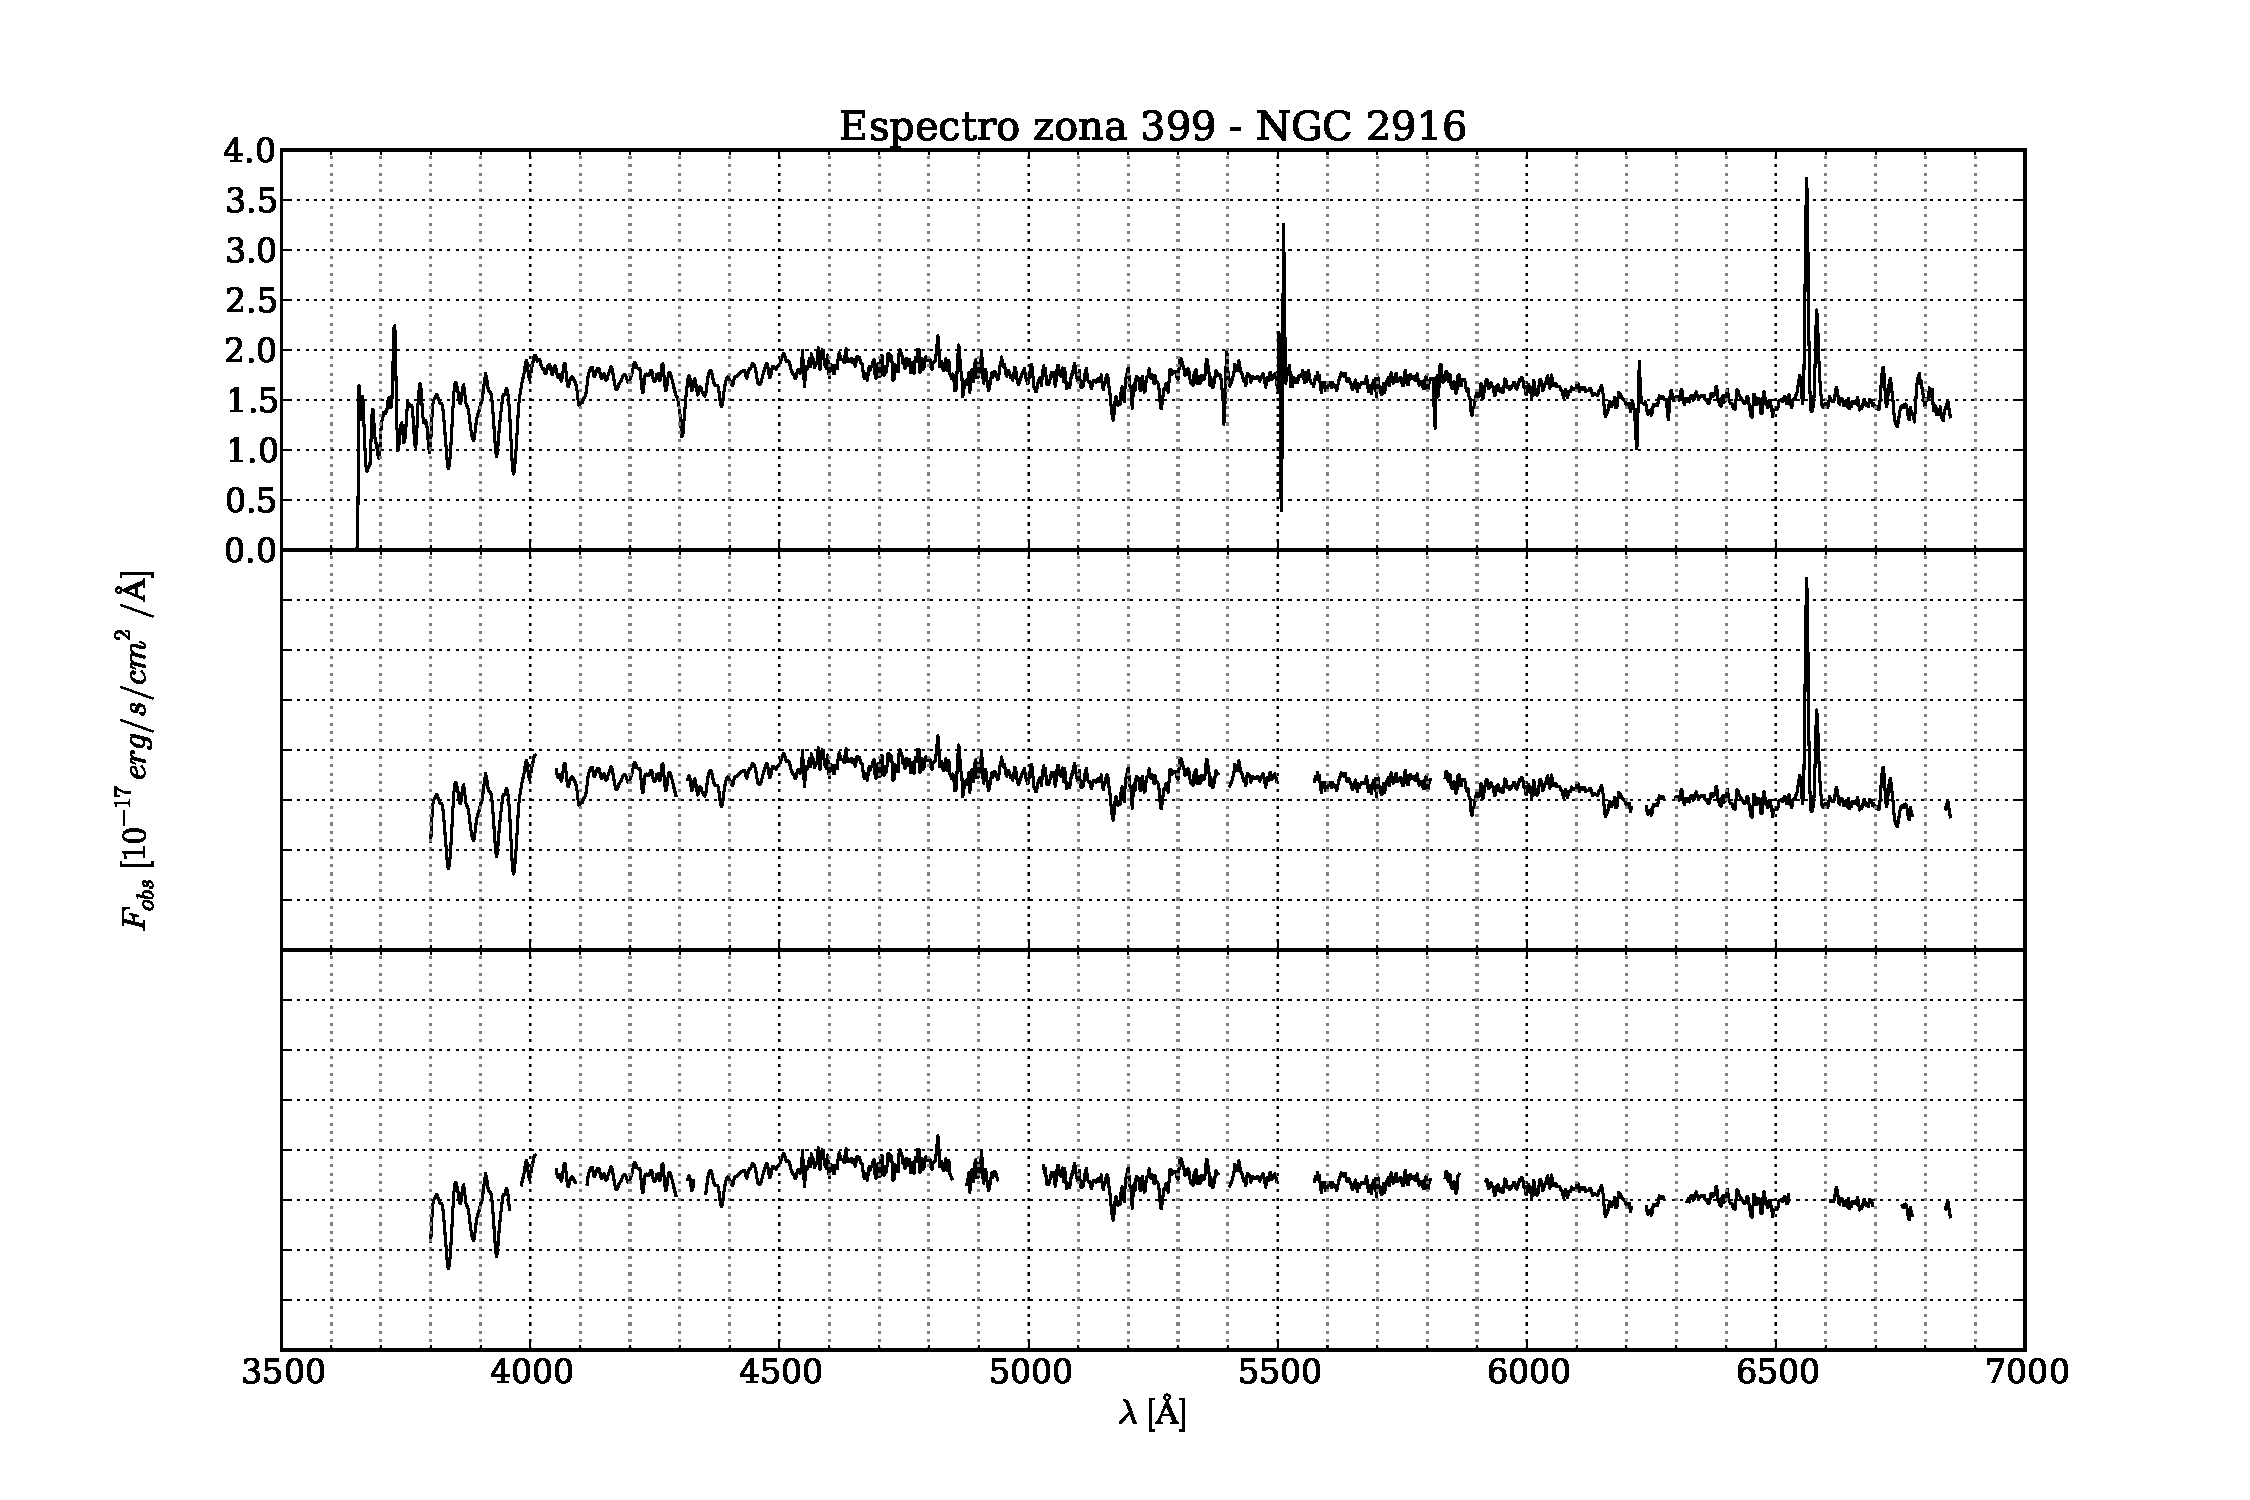
\includegraphics[width=1.0\textwidth]{figuras/K0277-constant_inital_mask-399.pdf}
    \caption[Exemplo de máscaras em um espectro do cubo de dados.]
    {Espectro da zona 399 da galáxia NGC 2916 (CALIFA 277). Acima está o espectro completo. No segundo vemos o espectro
    com linhas telúricas e bad-pixels removidos, além do limite de intervalo em comprimendo de onda de $3800$ a $6850$
    \AA. No espectro mais abaixo, além das partes removidas no segundo, estão foram removidas também as mesmas linhas de
    emissão mascaradas na síntese de populações estelares.}
    \label{fig:cap4:checkmask}
\end{figure}

\ldots \dots \ldots \ldots

Nos espectros, além dos {\em bad pixels} e linhas telúricas, podemos mascarar regiões desnecessárias para determinada
investigação científica. Nosso foco é o estudo das populações estelares, portanto necessitamos que as linhas de emissão,
geralmente associadas ao gás presente nas galáxias \fixme sejam removidas do espectro. Para que possamos fazer
correlações entre os resultados do PCA e as propriedades físicas obtidas pela síntese através do \starlight, em nossos
espectros também são mascaradas todas as regiões do espectro que não entram na síntese ($\mathrm{H}\epsilon$: de $3960$
a $3980$ \AA; $\mathrm{H}\delta$: de $4092$ a $4112$ \AA; $\mathrm{H}\gamma$: de $4330$ a $4350$ \AA; \Hbeta: de $4848$
a $4874$ \AA; \oIII: de $4940$ a $5028$ \AA; $\mathrm{He\,\textsc{i}}$ e $\mathrm{NaD}$: de $5866$ a $5916$ \AA; \Halpha
e \nII: de $6528$ a $6608$ \AA; $\mathrm{S\,\textsc{ii}}$: de $6696$ a $6752$ \AA). O espectro após todas máscaras pode
ser visto no terceiro espectro (o mais abaixo) da Figura \ref{fig:cap4:checkmask}.


\textcolor{red}{DAQUI PRA BAIXO AINDA É O ESQUELETO}
\ojo A Filosofia desse capítulo é aprender/testar como operar o PCA para que ele
reflita isso ou aquilo... descrevemos uma série de experimentos nesse sentido.

Preprocessamentos e diferentes tipos de PCAs com ou sem linhas, diferentes
faixas espectrais, com dados normalizados ou não. (importante!!!)

Vamos nos limitar a no-emission lines analysis, descrever a máscara de linhas de
emissão, etc. Isso para facilitar a coisa e pq queremos correlar o resultado do
PCA com os dados do Starlight (PyCASSO).

Simulações para ajudar a decifrar os resultador, população jovem + velha +
modelo de distribuição espacial - ver efeitos de estratégias de
preprocessamento.

Correlacionando os resultados do PCA com as propriedades do starlight (tipo de
engenharia reversa)

Linhas telúricas - remover ou não... bad pixels... mascarar ou não linhas de
emissão